\documentclass[preprint,12pt,authoryear]{elsarticle}

\usepackage{amssymb}
\linespread{1.2}

\usepackage{amsmath}
\usepackage{lineno}
\usepackage{graphicx}
\usepackage[colorlinks=true, allcolors=blue]{hyperref}
\usepackage[a4paper, total={6.in, 9in}]{geometry}
\linenumbers
\journal{Estuaries and Coasts}

%% NOTE (review): class is still elsarticle + elsarticle-harv. The Springer
%% template (sn-jnl/svjour3) + author-date bibliography switch is a separate
%% pending workstream and is NOT done here.

\begin{document}

\begin{frontmatter}

    \title{Seepage through the Sand Barrier at the Mouth of the Russian River, an Intermittently Closed Estuary}

\author[ars]{Octavia Crompton}
\affiliation[ars]{organization={USDA-ARS Hydrology and Remote Sensing Laboratory}}

\author[epa]{Dane Behrens}
\affiliation[epa]{organization={Environmental Science Associates, San Francisco}}

\author[bml]{John Largier}
\affiliation[bml]{organization={Bodega Marine Laboratory, Coastal \& Marine Sciences Institute, University of California Davis}}

\begin{abstract}
 Intermittently closed estuaries (ICEs) -- bar-built estuaries that periodically close --  are common along mountainous coastlines such as California's. While these estuaries provide valuable salmonid habitat, periodic closures can exacerbate challenges related to water quality and flood risk. Tools to forecast water levels during closures can support management decisions, such as whether to manually breach an estuary berm. One outstanding knowledge gap in the development of such tools is how much water seeps through the berm during closures.
Here, we estimate seepage rates through the berm of the Russian River estuary, a wave-dominated system in northern California that closes 1--15 times annually for 1--30 days. Using a mass-balance approach and Darcy's Law, we define an integrated hydraulic conductance, $C$, that captures the combined influence of the berm geometry and material properties. Across 32 closure events, seepage accounted for 20--60\% of river inflow, with average daily rates ranging from 0.5 to 3.0 m$^3$/s and $C$ values between 0.5 and 1.5 m$^2$/s. In some years, $C$ declined progressively over successive closures, suggesting seasonal clogging by fine sediments. Interannual variation in $C$ was associated with changes in berm shape following winter erosion and rebuilding. These results indicate that a linear head--seepage relationship provides an adequate operational approximation in the Russian River Estuary---although a model allowing conductance to vary with water level fits modestly better---and highlight how geomorphological and sedimentary changes jointly influence estuarine hydrodynamics.
\end{abstract}

\begin{highlights}
\item Berm seepage rates are quantified for an  intermittently-closed estuary in Northern California
\item The integrated hydraulic conductance of the berm decreases seasonally over subsequent inlet closures
\item Seepage accounts for 20-60\% of river discharge during inlet closures
\end{highlights}

\begin{keyword}
Intermittently closed estuaries \sep  Inlet closure \sep  Bar-built estuary \sep  Estuary water level
\end{keyword}

\end{frontmatter}

\section{Introduction}
\label{sec:intro}

In many smaller estuaries in Mediterranean climates and along mountainous coasts, the mouth is intermittently closed by a wave-built sand barrier \citep{mcsweeney2017intermittently, largier2023recognizing}.
These intermittently closed estuaries (ICEs) are common in California
\citep{heady2015assessing} and serve as important rearing habitats for juvenile salmonids \citep{bond2008marine, heady2015assessing, huber2020environmental}. Management options in these estuaries are often constrained by anthropogenic alterations of the physical system, including the development of adjacent low-lying flood-prone areas \citep{largier2019considerations}.

ICEs are typically found where estuary basins are small and the shore is exposed to high wave energy \citep{cooper2001geomorphological}. Closure events occur when wave power overwhelms the combined forces of river and tidal flows through the mouth \citep{behrens2013episodic, behrens2015quantified}.  This  is especially common in regions with weaker tides (micro-tidal and meso-tidal) and stronger wave action, such as the exposed coasts of California
\citep{mcsweeney2017intermittently}.
During dry-season periods of low river inflow, these small basins may lack sufficient tidal prism to maintain the mouth channel between the estuary and the ocean.
Peak water levels in these estuaries often occur during closed-mouth conditions \citep{booysen2020methods}, posing significant flood risks in developed floodplain areas adjacent to the estuary \citep{clark2019systematic}. However, such conditions can also play a critical role in sustaining wetlands as sea levels rise \citep{thorne2021wetlands}. Closures thus represent a critical management challenge in ICEs, where policy and management actions can alter closure frequency and persistence, with consequences for conservation, recreation, flooding, boating, and fisheries \citep{stein2021advancing}.

Long-term closure events in estuaries require a balance between water gains --through river inflow and wave-driven overwash -- and losses through evaporation and seaward seepage through the sand barrier.
In arid regions where river inflow is low and evaporation rates are high, evaporation can equal or exceed inflow, particularly in estuaries with larger surface areas \citep{largier2023recognizing}.
Alternatively, seaward flow over the barrier (overflow) can balance inflow, forming a `perched estuary', which can persist when overflow velocities are too weak to erode the barrier.
Another important, though less visible, mechanism for water loss is seepage through the sand barrier.
Here, we address the loss of water from a closed estuary via seepage, where  the head difference between estuary and ocean water levels drives water flows through the sand barrier \citep{perissinotto2010ecosystem}.
 Despite its importance in persistent closures and flood management in ICEs, seepage has received limited quantitative attention, representing a key knowledge gap.

The Jenner estuary at the mouth of the Russian river is one of many intermittently closed estuaries along California's coastline \citep{johnson1973characteristics, goodwin1996predicting, heady2015assessing}. The estuary has been monitored for many years, providing an opportunity to quantify seepage rates \citep{largier20205}.
River discharge is managed for water supply in summer and to mitigate flood risk in winter \citep{SonomaWater2011EIR}.
Management of the Russian River estuary requires balancing the habitat value for juvenile steelhead trout (O. mykiss) with the need to prevent high water levels that result in flooding during closure periods \citep{largier20205}. Historically, the river estuary opened and closed with the seasons.  However, due to flood risks posed to structures and farmland adjacent to the estuary, the berm is mechanically breached when estuarine water levels exceed 2.74 m NGVD29 (1.9 m NAVD88), following an inter-agency agreement (personal communication, Sonoma County Water Agency). Thus, artificial breaching typically limits the duration of estuary closures, and is known to impact estuarine habitats and downstream ocean ecosystems  \citep{largier2023recognizing, slinger2017modes}.  Very high water levels during closures are a potentially important source of accretion to marshes in outpacing sea level rise \citep{thorne2021wetlands}.

These tradeoffs between flood risk and marsh accretion highlight the need to better understand water loss mechanisms during closure periods. Here, we quantify water loss from the Russian River during 32 persistent closure events, using 12 years of compiled data on river flow rates and estuary and ocean water levels.
Using a mass balance approach, we estimate seepage rates during closure events and show that they increase with the head difference between estuary and ocean, consistent with Darcy-like flow through the berm.
We then define an integrated berm hydraulic conductance $C$ that reflects the combined influences of berm dimensions and material, and examine how $C$ varies seasonally and interannually.

\begin{figure}
    \centering
    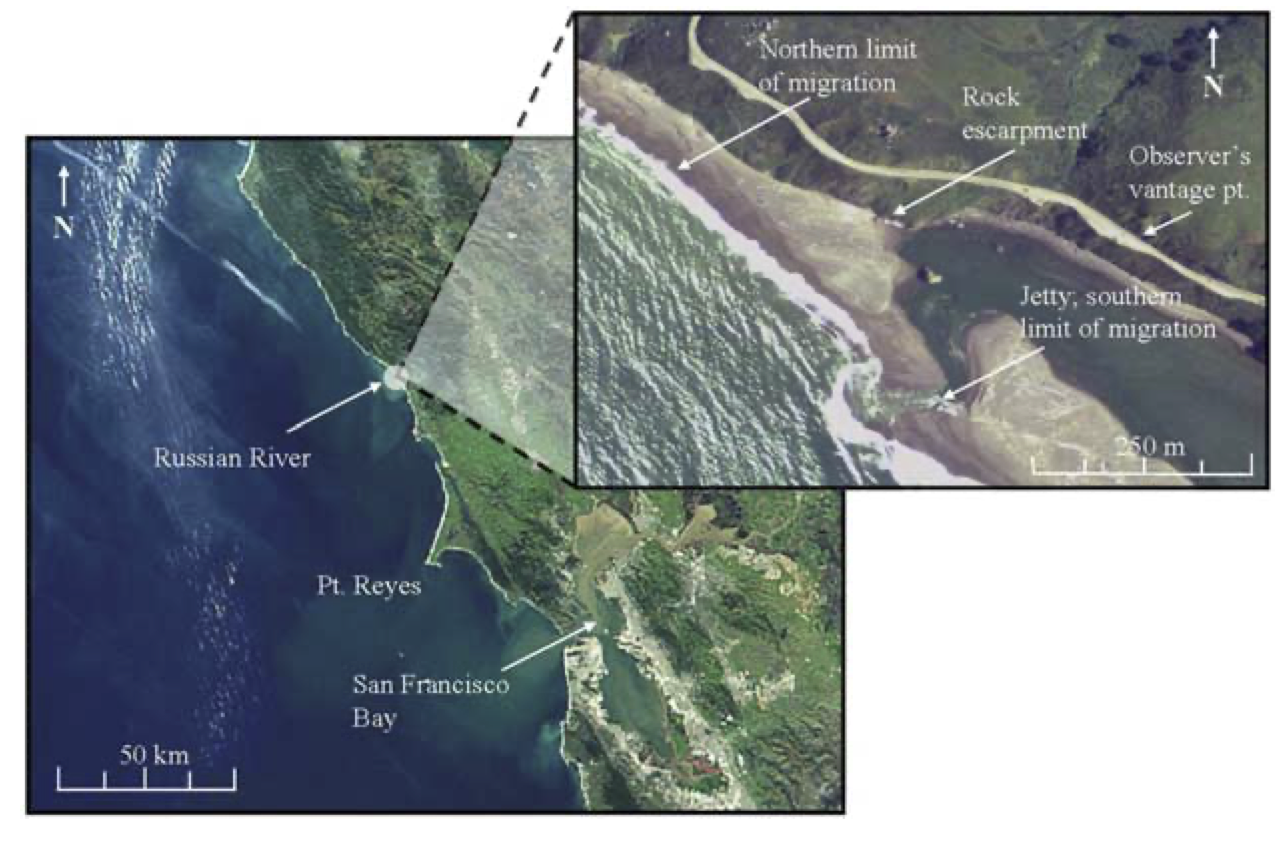
\includegraphics[width = 25pc]{figures/study_area.png}
    \caption{Location and physical characteristics of the study site. Image on the left available from NASA at \url{http:// visibleearth.nasa.gov/}.
    Location of inlet is at approximately 38\textdegree27'00''N, 123\textdegree07'00''W. Adapted from \citet{behrens2009characterization}.
    }
    \label{fig:study_area}
\end{figure}


\section{Methods}
\label{sec:methods}

\subsection{Study Area}
\label{sec:study_area}

The Russian River extends over 175 km within a basin of 3,850 km$^2$ and flows into the Pacific Ocean, 90 km north of San Francisco, California \citep[see Figure 1,][]{behrens2009characterization}. The region is characterized by a Mediterranean climate, with most precipitation falling during a handful of storms from November through April.  The area remains predominantly dry for the rest of the year.

The estuary closes between 1 and 15 times per year, with closure durations ranging from 1 to 30 days \citep{behrens2009characterization, largier20205}.
 These closures occur when the river current is unable to erode and remove sediment deposited in the inlet channel,  due to weakening river flows, insufficient tidal prism, and/or increasing frictional losses in the channel \citep{behrens2013episodic}.  Closures are most common during periods of high wave activity, low tidal ranges, and reduced river flow, with wave action playing a dominant role. In October--November, a seasonal increase in wave heights, combined with sporadic rainfall events and artificial breaching activity, often results in a series of inlet opening and closure events. Closures are ended by river inflows that fill the estuary basin,  raising the water level until it overflows and scours a new channel at a low point in the berm.
 The seasonality, frequency and persistence of closure events are expected to change in response to sea-level rise, as well as changes in wave power and river flow due to climate change.

\subsection{Data}

 Ocean water level data were obtained from the Point Reyes tide gauge operated by the National Oceanic and Atmospheric Administration (NOAA), located 48 km south of the inlet and representative of the ocean at the Russian River mouth. Within the estuary, a water-level gauge operated by the Sonoma County Water Agency, located 1.5 km upstream of the inlet, has collected hourly data  since 1999.
Additionally, a gauge operated by the U.S. Geological Survey (USGS) has provided real-time data 3 km from the mouth since 2018 (site no. 11467270).

We denote estuary water level at the Visitor Center gauge by $h(t)$ [m NAVD88] and ocean water level at the Point Reyes tide gauge by $h_{\mathrm{ocn}}(t)$ [m NAVD88]. The head difference driving seepage through the berm is then
\[
\Delta h(t) = h(t) - h_{\mathrm{ocn}}(t).
\]

Flow measurements are available from USGS stations at Hacienda Bridge (site no. 11467000), 27 km upstream of the inlet, and Austin Creek (site no. 11467200), located 11 km from the ocean inlet and the only perennial tributary to the lower river \citep{usgs_nwis_sw}.
These stations lie downstream of the Dry Creek confluence (capturing releases from Warm Springs Dam/Lake Sonoma), and downstream of the Wohler/Mirabel municipal diversion facilities operated by Sonoma Water \citep{sonomawater_watersupply}.  Consequently, $Q_r$  reflects upstream reservoir operations and municipal/irrigation diversions, and represents the net discharge that reaches the lower river and estuary \citep{SonomaWater_FishFlowDEIR_2016}.
These gauges have long, continuous records and are widely used as reference sites in Russian River hydrology and management studies \citep[e.g.,][]{anders2011water,newcomer2023prolonged}.
USGS water-data documentation indicates that daily-mean discharge records ratings typically have daily errors on the order of about 5--10\% \citep{USGS_WDR_Documentation_Explanation, Rantz1982_streamflow}.

The  estuary closure record is based primarily on webcam photos of the Jenner estuary collected by Bodega Marine Laboratory (see examples in Figure \ref{fig:closures}A).  Where images are unavailable (e.g., due to fog), closures can be inferred from the absence of tidal signature in the estuary gauge data, as illustrated by the timeseries of estuary and ocean levels  in Figure \ref{fig:closures}B.
Since 2012, there have been 107 closures, 63 with durations of 5 days or longer, and 30 with durations of 10 days or longer (see closure durations as a function of year in Figure \ref{fig:closures}C, and a histogram of closure event durations in Figure \ref{fig:closures}D).

\begin{figure}
    \centering
    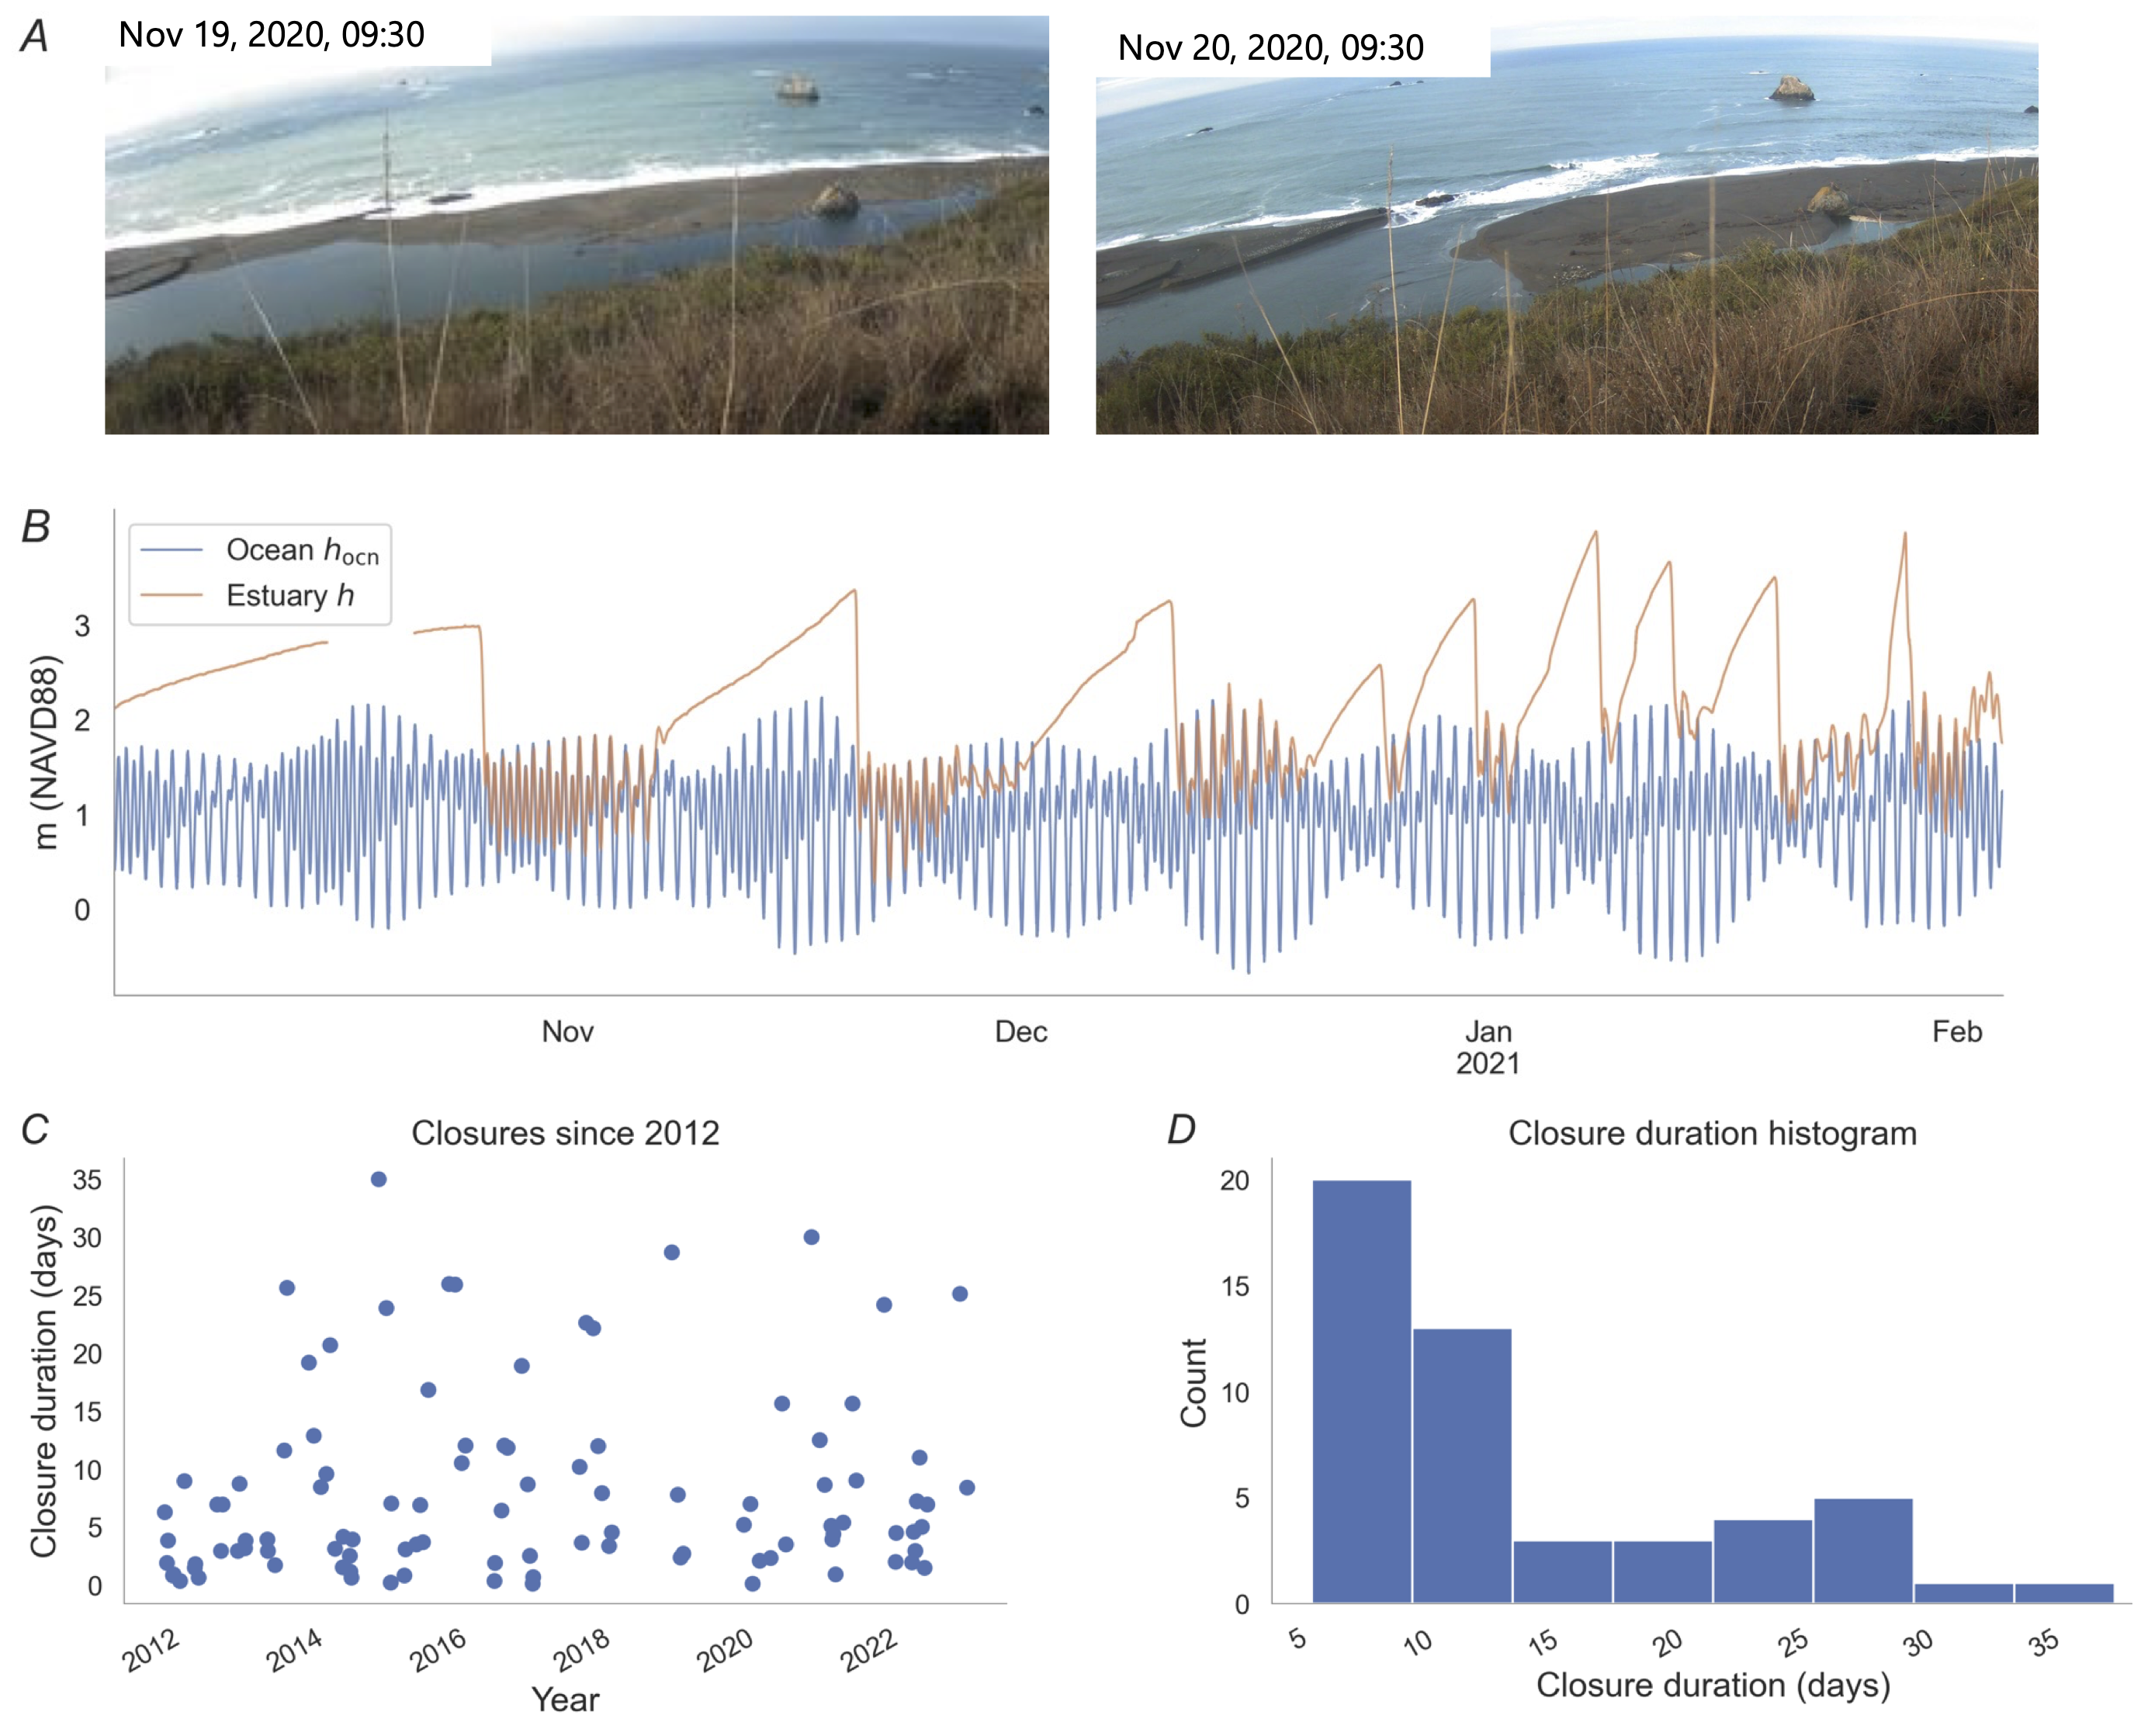
\includegraphics[width = \textwidth]{figures/fig3_closure_statistics.png}
    \caption{
    (A) Illustration of closed and open states of the estuary, showing the estuary closed on November 19, 2020 (left), and open the following day (right).
    (B) Example timeseries of water level $h$ for the estuary (orange) and ocean water level $h_{\mathrm{ocn}}$ (blue).
    (C) Closure duration (days) as a function of year for estuary closures from 2012 - 2023.
    (D) Histogram of closure durations (days) over the same 2012 - 2023 period.
    }
    \label{fig:closures}
\end{figure}

\begin{figure}
    \centering
    
\includegraphics[width = \textwidth]{figures/berm_schematic.png}
    \caption{Water balance and seepage at the closed Russian River estuary. (A) Cross-section showing the mass-balance terms (Equation~\ref{eq:dVdt}): gains (blue) from river discharge $Q_r$, wave overwash $O$, and precipitation $P$; losses (orange) from seepage $S$ and evaporation $E$; and net groundwater exchange $Q_{\mathrm{gw}}$ (grey). Inverted triangles mark the estuary stage $h$ and ocean level $h_{\mathrm{ocn}}$. (B) Seepage detail: the head difference $\Delta h = h - h_{\mathrm{ocn}}$ drives flow along the phreatic surface (dashed) through the barrier over flow-path length $L_b$ and saturated thickness $h_b$, giving $S = K\,A_b\,\Delta h / L_b$ with $A_b = W_b\,h_b$ (Equation~\ref{eq:Darcy}).}
    \label{fig:schematic}
\end{figure}

\subsection{Mass balance estimation of seepage rates}
\label{sec:MB}

We estimated the seepage rate, $S$ [L$^3$/T] at daily timesteps using a mass balance approach:

\begin{equation}
\label{eq:dVdt}
    \frac{dV}{ dt} = Q_r + P\,A_e(h) + O + Q_{\mathrm{gw}} - \big(S + E\,A_e(h) \big)
\end{equation}

\noindent  where $V$  represents the estuary volume [L$^3$],
$A_e(h)$   the estuary surface area at stage $h$ [L$^2$],
$Q_r$ the river discharge [L$^3$/T],
$P$ the precipitation rate [L/T],
$S$ the seepage through the berm [L$^3$/T],
$O$ wave-driven overwash [L$^3$/T],
$E$  the evaporation rate [L/T], and
$Q_{\mathrm{gw}}$ net groundwater exchange (positive into the estuary) [L$^3$/T]
and % $Q_{\mathrm{ov}}$ overflow across the berm [L$^3$/T]
(see schematic in Figure \ref{fig:schematic}).
Implicit in this mass balance is the assumption that groundwater-surface water exchanges are negligible and/or not persistent.
We computed $V$ as a function of estuary water level $h$ from a stage--volume (hypsometric) relationship derived from a 2011 bathymetric survey of the lower Russian River conducted for the Sonoma County Water Agency \citep{EDS_2011_LowerRussianRiver_Bathy}.
Figure \ref{fig:overwash}B illustrates the mass balance components for a 36-day closure from September 17 to October 22, 2014.
A daily timestep was used as travel times through berm are expected to be of the order of a day (estimated as $L_b/K$, with $L_b \approx 50$ m and sand $K \approx$ 45 m/day), thus smoothing out the effect of tidal, diurnal and other high-frequency fluctuations on seepage rate.

To identify upper limits of daily evaporation from the estuary, we estimated the estuary area as 1 km$^2$ and the maximum  evaporation rate as 10 mm/day, which yields $E A_e(h) \approx 0.1$ m$^3$/s. Accordingly, we did not include evaporation in the analysis, because this term is likely an order of magnitude smaller than typical river discharge during closures ($Q_r \approx 1-5$ m$^3$/s).  Precipitation was retained in the mass balance using daily rainfall records from the nearby Bodega Marine Laboratory station, converted to a volumetric flux as $P\,A_e(h)$; because the analyzed closures occur during the dry season, this term contributed negligibly to the seepage estimate (less than 0.3\% of $S$ on every analyzed day). Groundwater exchange and cross-berm overflow were neglected during the analyzed closure days.

With these simplifications, rearranging Equation \ref{eq:dVdt} yields:

\begin{equation}
\label{eq:S}
    S  = Q_r + P\,A_e(h) - \frac{dV}{ dt} + O.
\end{equation}

Preliminary analyses showed occasional days with  $Q_r - \frac{dV}{ dt} <0$, i.e., days in which the estuary volume increased more than river discharge can account for, which we attribute to wave overwash. Overwash can occur on days with big waves at high tide and is most common near the beginning of closures events (i.e., within the first couple of days, before wave action builds up the sand barrier crest elevation).

To exclude days with overwash, we applied a filtering approach that used river discharge $Q_r$ to forecast estuary depth on the following day. Specifically, river discharge and  estuary volume  on day $t$ were used to predict the estuary volume on the following day,  as $\hat V_{t+1} = V_{t} + Q_{r,t} \Delta t$.    $\hat h_{t+1}$  was then calculated from $\hat V_{t+1}$ using hypsometry data.
If seepage, evaporation, and overwash are all negligible, we expect that $h_{t+1} = \hat h_{t+1}$. If overwash is negligible and seepage is significant, then $ h_{t+1} < \hat h_{t+1} $. Conversely, if  the overwash  exceeds seepage, then $h_{t+1} > \hat h_{t+1} $.  To exclude overwash days, we removed days with $h_{t+1} > \hat h_{t+1}$ and $Q_r - \frac{dV}{ dt} < 0$ from the analysis (e.g., Figure 4C: September 18-19 and 25-26, and October 12-13).
 Excluding days with  $ h_{t+1} > \hat h_{t+1}$ is a more restrictive criteria than the simpler approach of excluding days with $Q_r - \frac{dV}{ dt} < 0$.
Visual inspection of estuary photographs confirmed overwash on all excluded days.

 With these days filtered out, we assumed that overwash was negligible on the remaining days ($O \sim 0$); however, there may be weaker overwash on other days that reduces the estimate of seepage $S$ (e.g., Figure 4C: 20 September). Under the assumption of negligible overwash, Equation \ref{eq:S} simplifies to:

\begin{equation}
    S  = Q_r + P\,A_e(h) - \frac{dV}{ dt}.
\end{equation}

  \begin{figure}
    \centering
    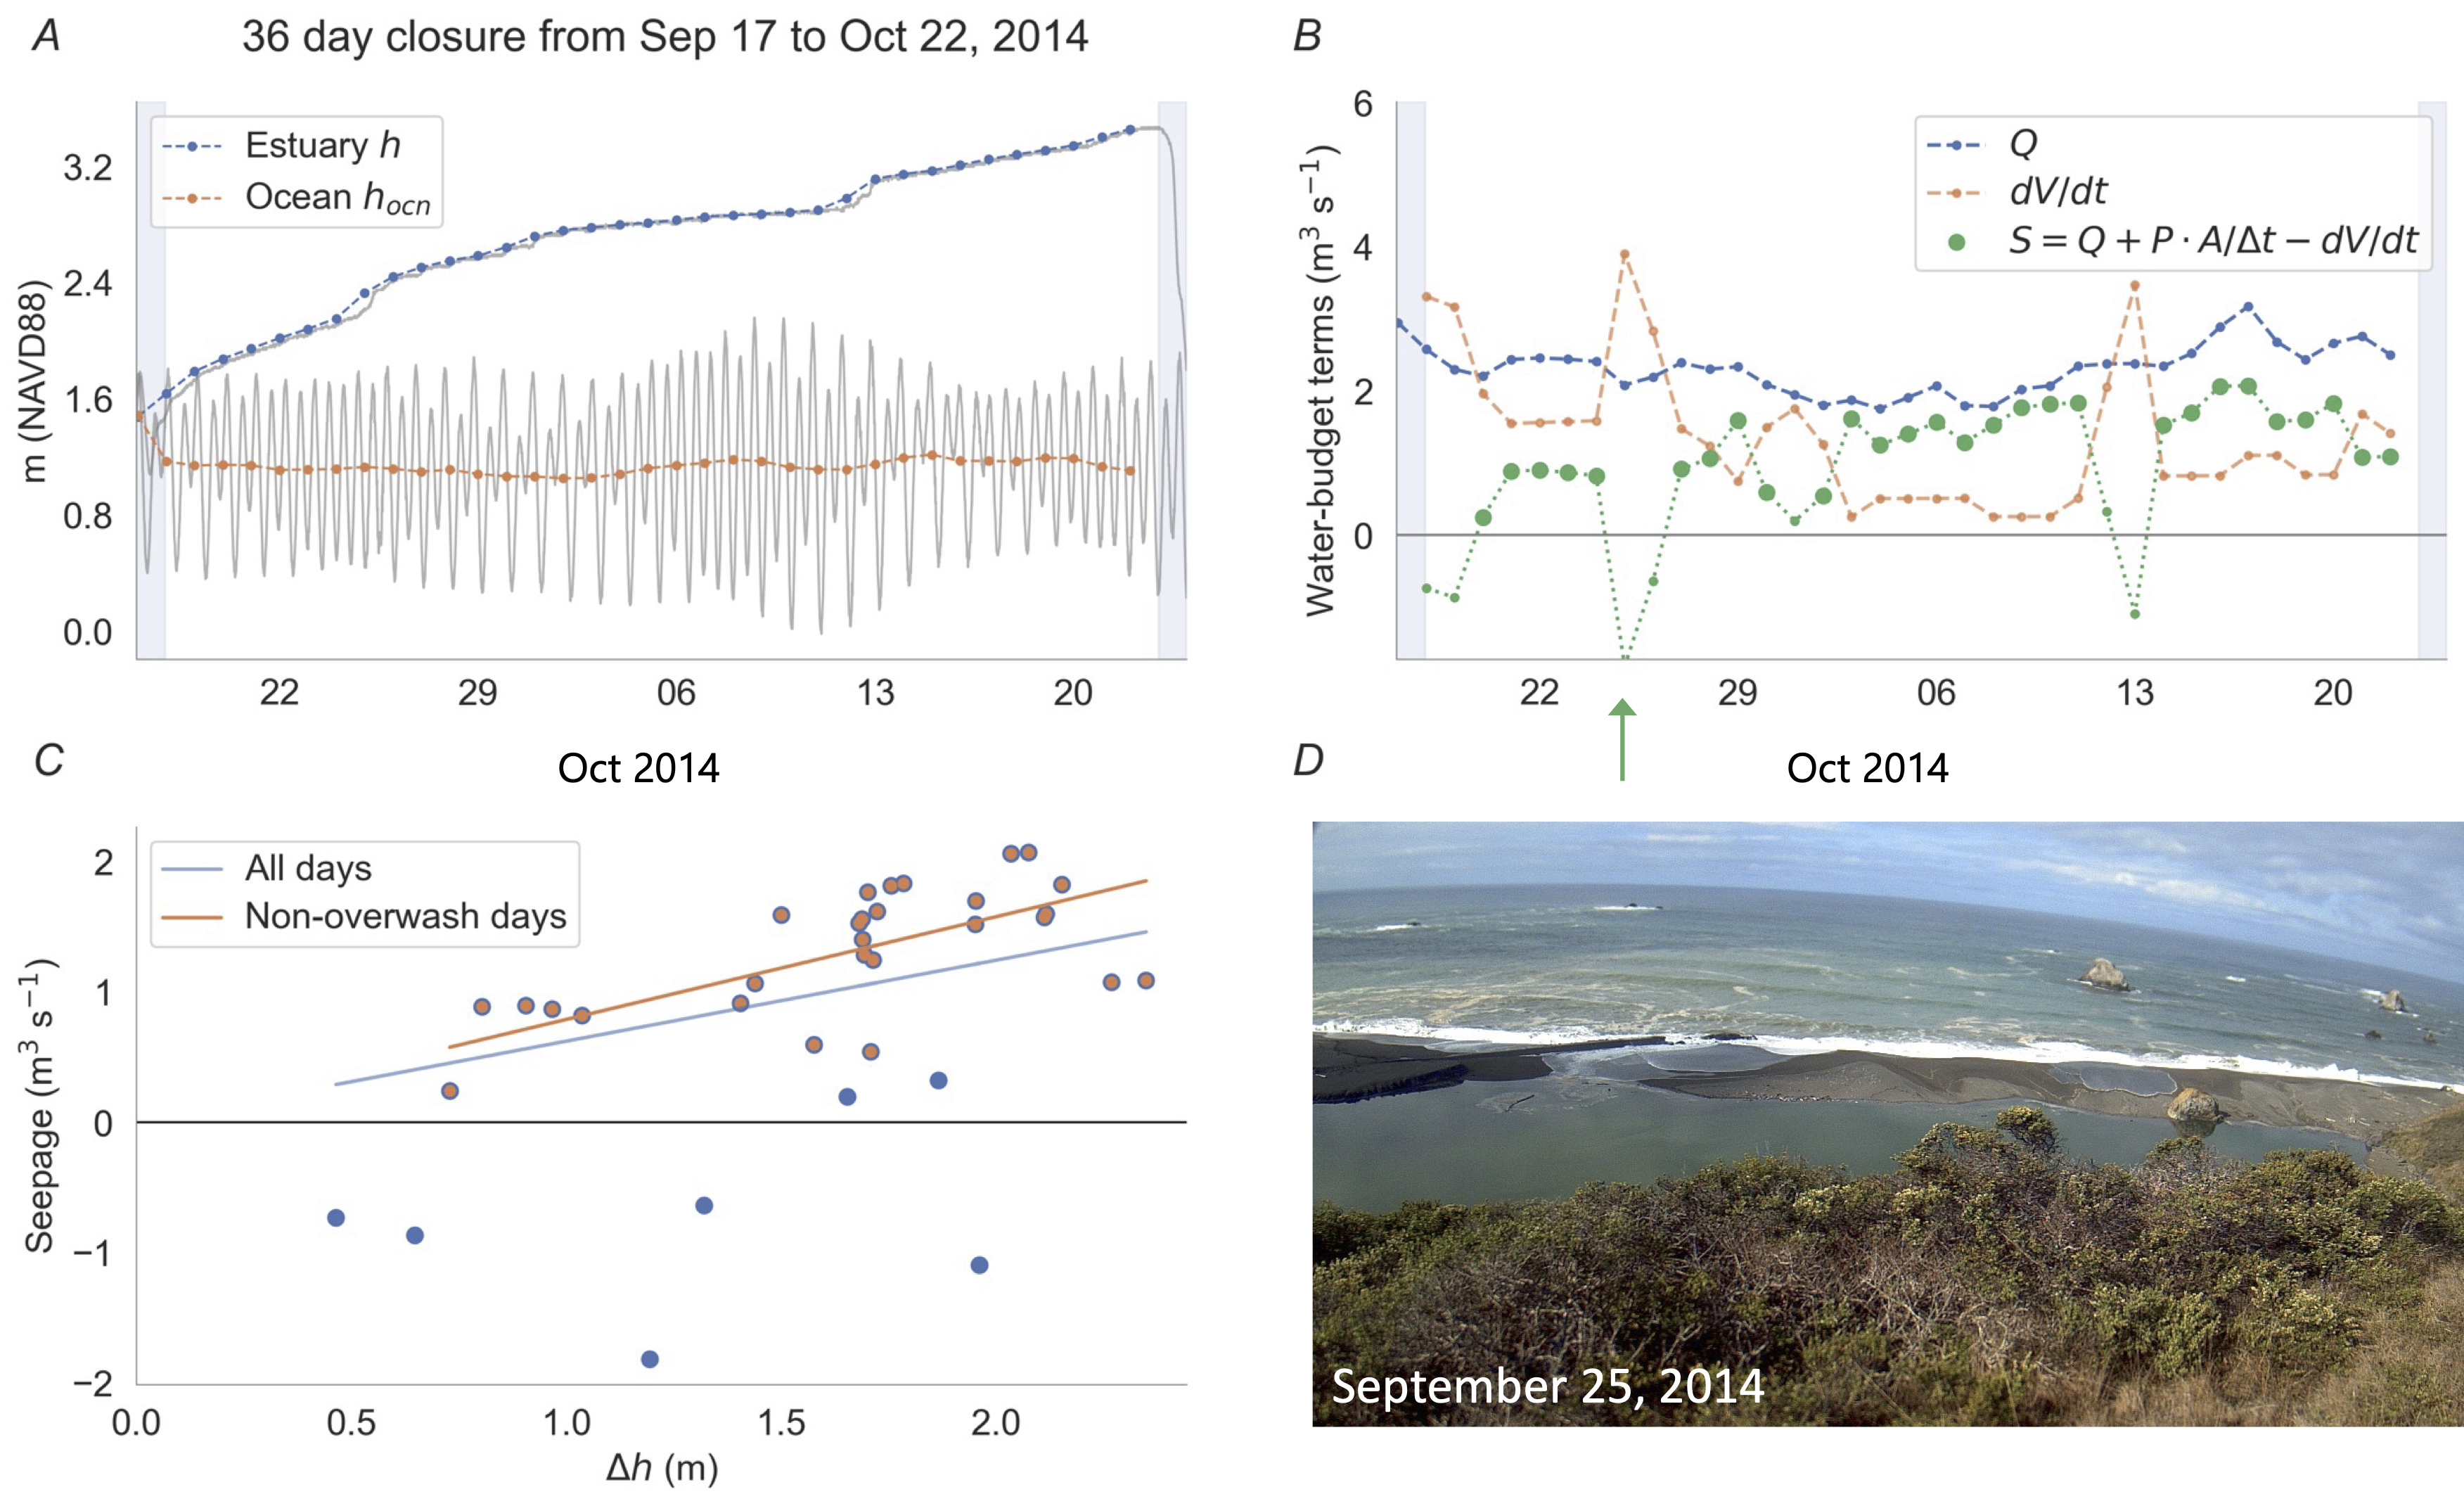
\includegraphics[width = \textwidth]{figures/fig4_overwash.png}
    \caption{(A) Timeseries of estuary water level $h$ and ocean level $h_{\mathrm{ocn}}$ during a closure from September 17 to October 22, 2014.
    Solid lines show 15 minute data, and dotted lines show the daily averaged data. Grey shading indicates periods when the estuary mouth was open.
    (B) The mass balance components at daily intervals: the estuary volume change per day, $dV/dt$  (orange),  river discharge, $Q_r$  (blue) and seepage, $S = Q - dV/dt$ (green). In the $S$ timeseries, smaller marker sizes indicate points that were filtered out to exclude days dominated by overwash. (C) The berm integrated hydraulic conductance $C_L$ was computed by fitting a regression of $S$ on $\Delta h$ for days not excluded as overwash (see Section \ref{sec:MB}).
    (D) A photo of the estuary mouth taken September 25, 2014, in which overwash is visible.
    }
    \label{fig:overwash}
\end{figure}


\subsection{Integrated berm hydraulic conductance}

We assume that Darcy's law applies to seepage across the berm:

\begin{equation}
    S = K A_b \frac{\Delta h}{ L_b}
    \label{eq:Darcy}
\end{equation}

\noindent where $K$ [L/T] is the mean hydraulic conductivity of the berm, $\Delta h = h - h_{\mathrm{ocn}}$  [L] is the head difference between estuary and ocean, $A_b$ [L$^2$] is the cross-sectional berm area, and $L_b$ [L] is the berm width between estuary and ocean (the distance over which hydraulic pressure drops from estuary to ocean). More precisely, $A_b = W_b h_b$ is the hydraulically active cross-sectional area of flow,  where $W_b$ and $h_b$ are the along-shore width and vertical height, respectively, of water flow through the berm.

As the estuary water level rises, the hydraulic gradient increases, and the berm geometry may itself change: a higher estuary stage can thicken the saturated cross-section $A_b$ and shorten the flow path $L_b$, so that the ratio $A_b/L_b$ --- and hence the conductance --- may increase with stage. Because $A_b$ and $L_b$ are not directly observable and their dependence on stage is unknown, we absorb the geometry into an effective hydraulic conductance $C$:

\begin{equation}
    S = C\,\Delta h,
    \label{eq:tildeK}
\end{equation}

\noindent where $C = K\,A_b/L_b$. While the berm shape can be estimated from aerial or satellite imagery, this likely differs from its hydraulically-active area.

%% --- Power-law (geometric) derivation of the stage dependence, retained for reference; ---
%% --- NOT rendered in the live text. Can be reinstated if a reviewer requests it.        ---
%% Let h_e denote estuary water DEPTH (the physically relevant quantity governing the berm
%% geometry), related to the gauge level h by   h_e = h + \delta_V ,  where \delta_V offsets
%% the NAVD88 datum (h = 0 near mean low tide) to the effective base of the flow path.
%% SIGN: the relation is PLUS \delta_V, matching the code ( \zeta_V = (h + \delta_V)/m_V ).
%% The fitted \delta_V is negative (~ -1.72 m), so h_e = h + \delta_V behaves as a THRESHOLD
%% ( h_e -> 0 at gauge level h = -\delta_V ~ 1.72 m ), not a positive depth datum.
%% Writing the geometry as power laws in depth:
%%   A_b = A'_b h_e^x ,   L_b = L'_b h_e^y        (x > 0: area grows; y < 0: path shortens)
%%   S = K (A'_b h_e^x) \Delta h / (L'_b h_e^y) = K (A'_b/L'_b) h_e^{x-y} \Delta h
%% so the effective conductance C = K A'_b/L'_b and the exponent b_V plays the role of (x - y):
%%   S = C_V \zeta_V^{b_V} \Delta h ,  with  \zeta_V = (h + \delta_V)/m_V = h_e / m_V .
%% ----------------------------------------------------------------------------------------------

Because mouth-scale geometry is unavailable and the analysis is restricted to closed-mouth periods, we do not model the berm dimensions $A_b$ and $L_b$ explicitly. Instead, we treat the geometric factor $A_b/L_b$ in Equation~\ref{eq:tildeK} as an empirical function of estuary stage and test whether the gauge level $h$ serves as a proxy for it, comparing a constant-conductance (linear) model with a nonlinear model in which the conductance varies with stage.

Because the berm geometry responds to water depth within the barrier, whereas the gauge level $h$ is referenced to the NAVD88 datum ($h = 0$ near mean low tide), and the active seepage cross-section need not vanish at $h = 0$, we introduce an additive offset $\delta_V$ so that $(h + \delta_V)$ serves as the depth-like stage variable governing $A_b/L_b$.

Because $h$ and $\Delta h$ share the estuary-stage component, the conductance modulator $\zeta_V(h)$ and the driving head $\Delta h$ are not fully independent; the ocean term in $\Delta h$ contributes mainly tidal variance.

We compare two forms for the seepage--head relationship. The first is a linear, constant-conductance model, $S = C_L\,\Delta h$, in which the conductance $C_L$ does not vary with stage. The second allows the conductance to vary with estuary water level through a nonlinear (offset-power) form,
\begin{equation}
  S \;=\; C_V\,\zeta_V^{\,b_V}\,\Delta h,
  \qquad
  \zeta_V = \frac{h + \delta_V}{m_V},
  \qquad
  m_V = \mathrm{median}(h) + \delta_V,
  \label{eq:offsetpower}
\end{equation}
where $\zeta_V$ is a dimensionless scaled water level and $m_V$ is its median normalization, so that $C_V$ retains units of conductance and equals the effective conductance at median stage (i.e., where $\zeta_V = 1$). The exponent $b_V$ sets how strongly conductance varies with stage: a positive $b_V$ corresponds to a seepage cross-section that grows, and/or a flow path that shortens, as the estuary fills. The offset $\delta_V$ locates the effective stage datum of this modulation; a negative $\delta_V$ implies a threshold stage, $h = -\delta_V$, below which the conductance factor approaches zero. The linear model is the special case $b_V = 0$, for which $\zeta_V^{\,b_V} = 1$ and $S = C_L\,\Delta h$.

We fit the linear model both pooled (one $C_L$ from all closure days) and per event (a separate $C_L$ for each closure), in each case by through-origin ordinary least squares regression of $S$ on $\Delta h$ (see Figure~\ref{fig:overwash}C for illustration). Per-event linear fits were restricted to closures with at least five daily data points ($N \ge 5$), which provides at least four residual degrees of freedom for the through-origin fit and enough points to bootstrap a within-event 95\% confidence interval on $C_L$; the seasonal pattern in $C_L$ is insensitive to raising the threshold to $N \ge 6$ or $N \ge 8$.
The nonlinear model was fit at the pooled level, estimating $C_V$, $\delta_V$, and $b_V$ by minimizing the sum of squared residuals, with $\delta_V$ constrained so that $h + \delta_V > 0$. Per-event nonlinear fits are not reported, because the three free parameters are weakly identified within individual closures; the per-event panels of Figure~\ref{fig:compare_fits} (A--C) therefore show only the per-event linear fit, while the pooled nonlinear fit is shown alongside the pooled linear fit in panel D.

Model performance was evaluated using the Akaike and Bayesian Information Criteria (AIC, BIC), computed as
\begin{equation}
    \mathrm{AIC} = n \cdot \ln(\mathrm{SSE}/n) + 2k,
    \qquad
    \mathrm{BIC} = n \cdot \ln(\mathrm{SSE}/n) + k \ln n,
\end{equation}
where $n$ is the number of observations, $\mathrm{SSE}$ is the sum of squared residuals, and $k$ is the number of model parameters ($k = 1$ for the linear model, $k = 3$ for the nonlinear model). Lower values indicate a more parsimonious model. We report the pooled AIC and BIC and assess goodness of fit with the centered coefficient of determination, $R^2$.


\section{Results}

Table~\ref{tab:closures} lists the linear conductance $C_L$ (with bootstrapped 95\% confidence intervals) and goodness of fit $R^2_L$ for each closure with at least five daily data points ($N \ge 5$). Figure~\ref{fig:compare_fits} compares the linear and nonlinear fits for the three longest closures (panels A--C) and for all closure days pooled (panel D).
In the pooled fit, both AIC and BIC favor the nonlinear model over the linear model ($\Delta\mathrm{AIC} = -18.4$, $\Delta\mathrm{BIC} = -10.4$).
However, the improvement in prediction error is modest: the pooled $R^2$ increases from 0.45 (linear) to 0.48 (nonlinear), a bootstrapped mean gain of $\Delta R^2 = +0.030$ (95\% CI $[0.013,\,0.055]$).
Given the comparable errors, the linear model $S = C_L\,\Delta h$ provides a parsimonious baseline, while the nonlinear model captures additional structure in the conductance--water-level relationship.

  \begin{figure}
    \centering
    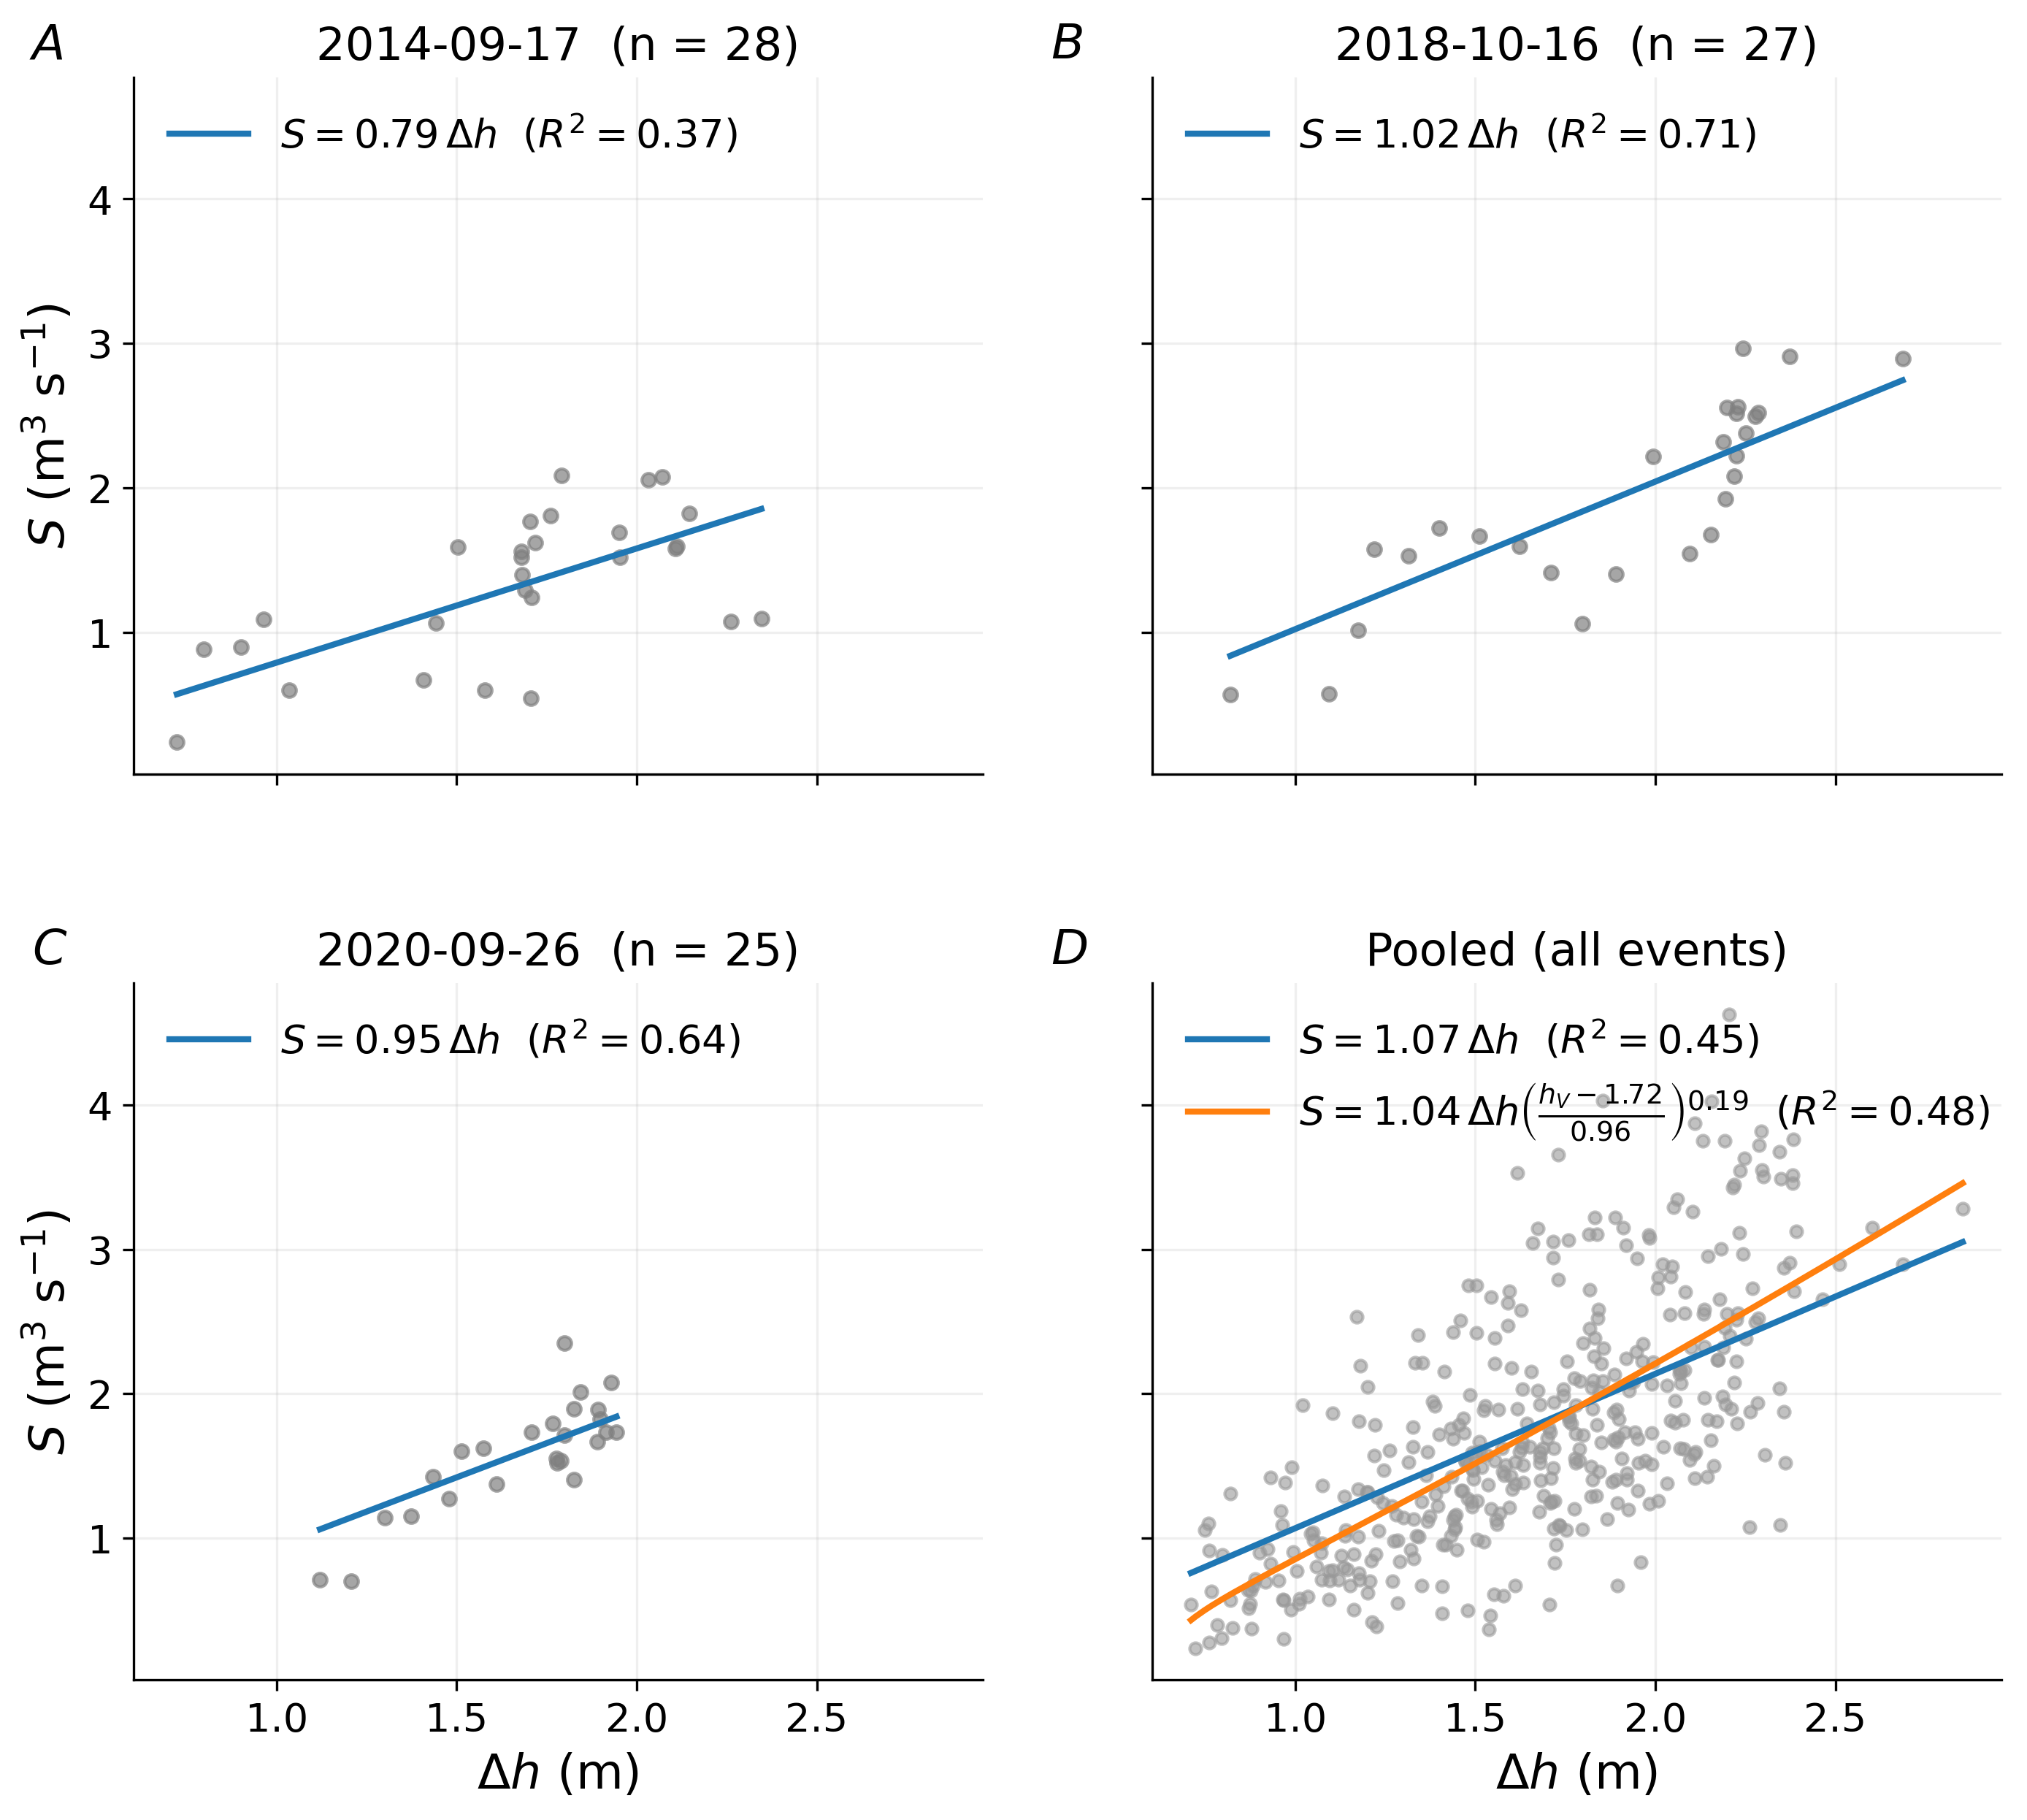
\includegraphics[width = 0.8\textwidth]{figures/fig5_model_comparison_panels.png}
    \caption{Comparison of seepage--head model fits for the three longest closures and for all closure days pooled. Panels (A)--(C) show the per-event linear fit (blue) for each closure: (A) a 36-day closure starting September 17, 2014 (see also Figure \ref{fig:overwash}); (B) a 29-day closure starting October 16, 2018; (C) a 31-day closure starting September 26, 2020. (D) All closure days pooled, showing the pooled linear fit (blue) and the pooled nonlinear fit (orange). Panels B and C are shown in further detail in SI Figures S1 and S2 (analogous to Figure \ref{fig:overwash}). Axes: $\Delta h$ (m) versus $S$ (m$^3$ s$^{-1}$).
    }
    \label{fig:compare_fits}
\end{figure}

\begin{figure}
    \centering
    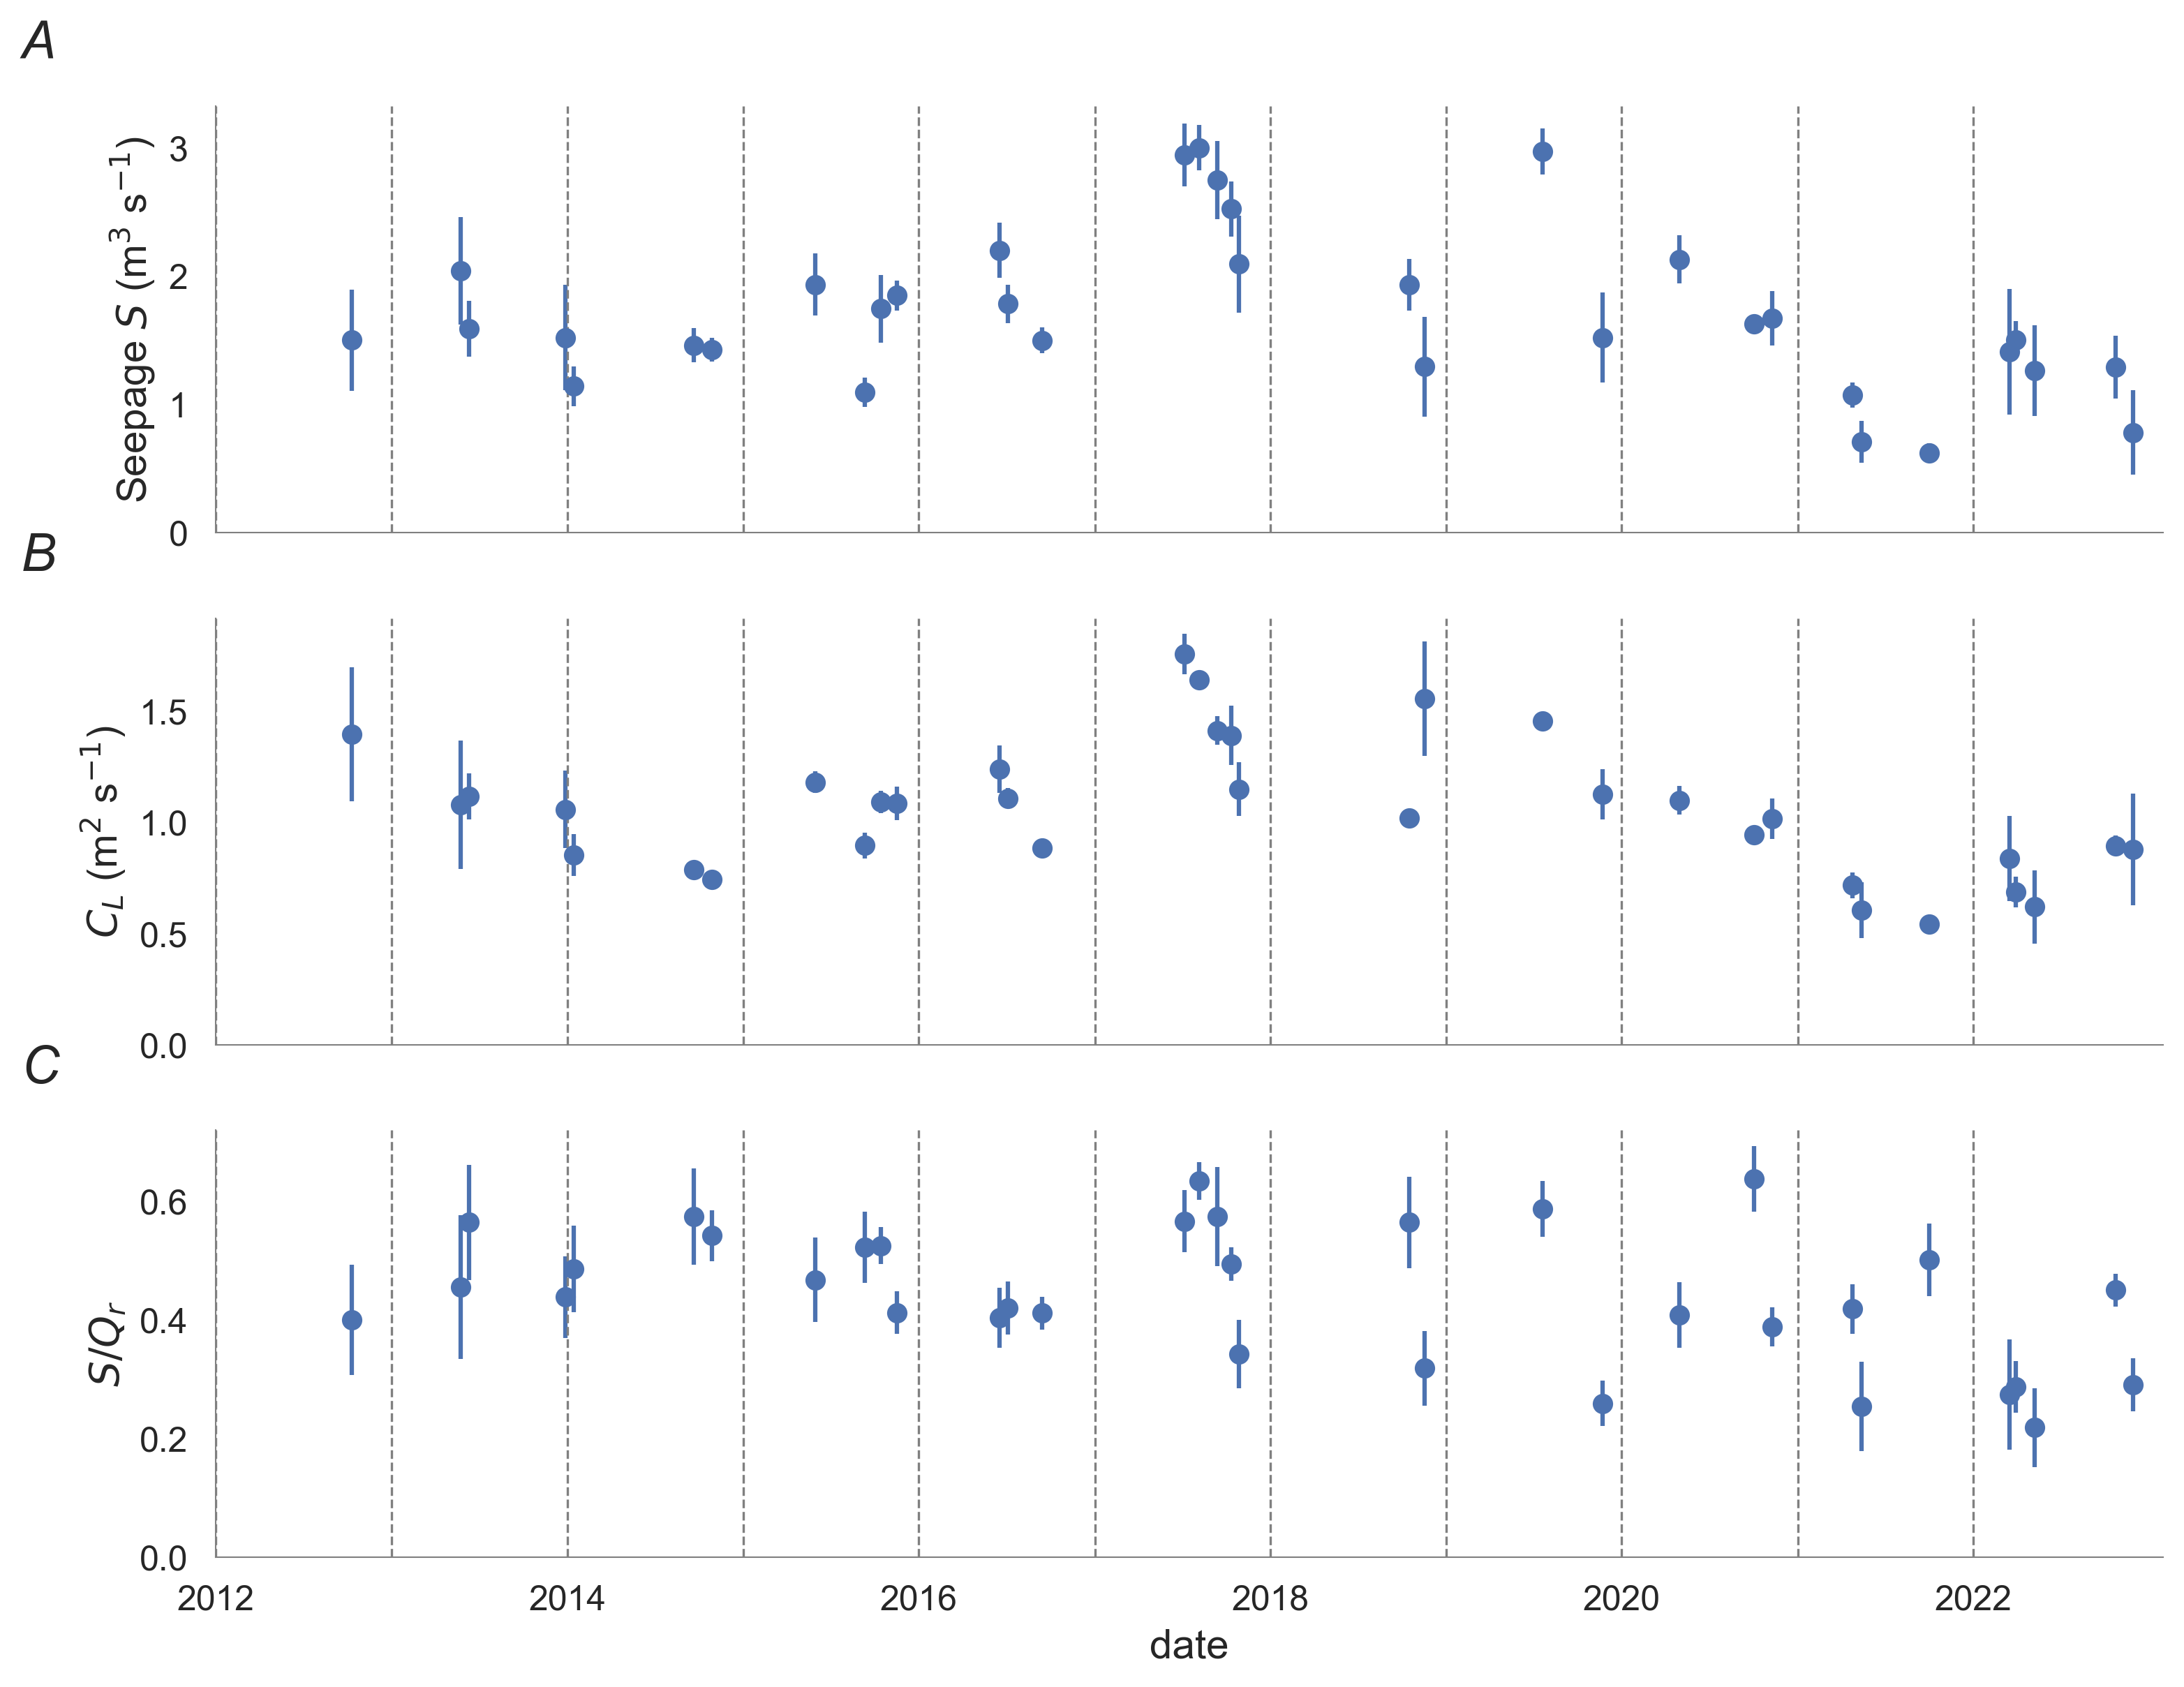
\includegraphics[width = \textwidth]{figures/summary.png}
    \caption{(A) Mean seepage rate $S$ (m$^3$ s$^{-1}$) computed for each closure, with error bars indicating bootstrapped confidence intervals on the mean.
    (B) Integrated hydraulic conductance $C_L$ (m$^2$ s$^{-1}$) determined through regression of $S$ on $\Delta h$ for each closure event.
    (C) Ratio of seepage to river discharge, $S/Q_r$.
    Only closure events with at least five daily data points ($N \ge 5$) are included.
    }
    \label{fig:summary}
\end{figure}

Figure \ref{fig:summary} shows how the mean seepage rate $S$  (panel A) and the integrated hydraulic conductance $C_L$ (panel B) vary over time for all closures with at least five daily data points ($N \ge 5$). Seepage rates vary from 0.5 to 3.0 m$^3$/s, with the highest rates in 2017. $C_L$ remains relatively consistent across closures, ranging from 0.5 to 1.5 m$^2$/s. The highest conductance was observed in 2017, consistent with the  high seepage rates that year. In some years, $C_L$ decreases over subsequent closures (notably, in 2016 and 2017), reflecting a seasonal change in $K$, $A_b$, and/or $L_b$.
Figure \ref{fig:summary}C shows the ratio of seepage to river discharge, $S/Q$, which ranges from 0.2 to 0.6, with significant variability both within and between years.

Supporting information Figure S3 compares the results obtained with and without overwash days included in the analysis (i.e., $S$ versus $S + O$). If the data are not filtered to exclude days with wave-driven overwash, $C_L$ represents an integrated hydraulic conductance representing both seepage and overwash, $S + O$. $C_L$ values are smaller with overwash included, because the net water loss $O + S$ can underestimate the actual seepage $S$ when overwash offsets part of the volume change.
Nevertheless, the results are qualitatively similar, showing the same seasonal and interannual trends in $C_L$.

\begin{table}[]
    \centering
\caption{Per-event linear seepage fits for all 32 closures with at least five daily data points ($N \ge 5$), listing closure start date, duration (days), and number of daily data points $N$. $C_L$ is the conductance of the linear model $S = C_L\,\Delta h$, with bootstrapped 95\% confidence intervals (resampling daily values within each closure), and $R^2_L$ is the corresponding coefficient of determination. Because the model passes through the origin, $R^2_L$ can be negative for closures with little range in $\Delta h$.}
    \small
\begin{tabular}{lll|lll}
\hline
date & duration & $N$ & $C_L$ & 95\% CI & $R^2_L$ \\
\hline
2014-09-17 & 36 & 28 & 0.79 & [0.70, 0.88] & 0.37 \\
2020-09-26 & 31 & 25 & 0.95 & [0.90, 1.00] & 0.64 \\
2018-10-16 & 29 & 27 & 1.02 & [0.96, 1.09] & 0.71 \\
2015-09-08 & 27 & 23 & 0.90 & [0.79, 1.00] & 0.04 \\
2015-10-10 & 27 & 21 & 1.09 & [1.00, 1.16] & 0.79 \\
2022-10-21 & 26 & 18 & 0.93 & [0.84, 1.03] & 0.72 \\
2013-06-08 & 26 & 17 & 1.18 & [0.94, 1.39] & 0.37 \\
2014-10-24 & 25 & 21 & 0.75 & [0.69, 0.80] & 0.52 \\
2021-09-28 & 25 & 17 & 0.56 & [0.50, 0.62] & 0.58 \\
2017-08-05 & 23 & 22 & 1.66 & [1.60, 1.72] & 0.86 \\
2017-09-12 & 23 & 20 & 1.42 & [1.30, 1.52] & 0.58 \\
2014-01-11 & 22 & 10 & 0.87 & [0.67, 1.08] & 0.53 \\
2016-09-11 & 19 & 17 & 0.88 & [0.80, 0.97] & 0.36 \\
2015-05-28 & 18 & 15 & 1.18 & [1.08, 1.25] & 0.79 \\
2020-04-29 & 16 & 15 & 1.11 & [0.98, 1.26] & 0.61 \\
2021-04-21 & 16 & 13 & 0.72 & [0.63, 0.83] & 0.41 \\
2020-11-07 & 13 & 11 & 1.00 & [0.84, 1.12] & 0.65 \\
2016-06-15 & 13 & 10 & 1.25 & [1.09, 1.48] & -0.04 \\
2017-10-07 & 13 & 9 & 1.39 & [1.15, 1.55] & 0.51 \\
2022-03-28 & 12 & 9 & 0.83 & [0.69, 1.04] & 0.22 \\
2016-07-01 & 12 & 8 & 1.14 & [1.08, 1.18] & 0.87 \\
2013-05-23 & 12 & 5 & 1.08 & [0.57, 1.53] & 0.17 \\
2015-11-13 & 11 & 8 & 1.09 & [0.98, 1.21] & 0.57 \\
2017-07-04 & 11 & 8 & 1.82 & [1.68, 1.98] & 0.54 \\
2022-11-25 & 10 & 6 & 1.05 & [0.64, 1.33] & 0.54 \\
2013-12-23 & 10 & 5 & 1.03 & [0.77, 1.23] & 0.43 \\
2021-05-10 & 10 & 5 & 0.89 & [0.47, 1.53] & 0.04 \\
2012-10-07 & 9 & 5 & 1.26 & [1.10, 1.36] & 0.75 \\
2018-11-16 & 9 & 5 & 1.51 & [1.08, 1.82] & 0.48 \\
2019-11-20 & 8 & 6 & 1.38 & [1.03, 1.77] & 0.56 \\
2017-10-25 & 8 & 5 & 1.15 & [0.98, 1.29] & 0.73 \\
2022-03-14 & 8 & 5 & 0.82 & [0.49, 1.08] & 0.36 \\
\hline
\end{tabular}
    \label{tab:closures}
\end{table}


\section{Discussion}

Water loss from the Russian River estuary via seepage through the sand barrier increases with increasing head difference $\Delta h$ (see Figure \ref{fig:compare_fits}). A model comparison indicates a weak dependence of the effective conductance on estuary water level: the nonlinear model is statistically favored over the constant-conductance model ($\Delta\mathrm{AIC} = -18.4$, $\Delta\mathrm{BIC} = -10.4$), but the fitted exponent is small ($b_V \approx 0.19$) and the gain in explained variance is modest (pooled $R^2$ of 0.45 versus 0.48). A small positive $b_V$ implies that rising estuary water level only weakly increases the ratio of cross-sectional flow area to flow length, $A_b/L_b$ -- either because $A_b$ and $L_b$ depend weakly on water level, or because their dependencies approximately offset. Alternatively, the weak level-dependence of conductance may reflect a preferred conduit for seepage whose geometry changes little as the estuary fills. We emphasize that these inferences are specific to the Russian River berm and carry the uncertainties inherent in a residual-based mass balance (discussed below); the near-linear dependence of seepage on head difference found here may not generalize to other ICEs, where barrier dimensions, sediment composition, and legacy structures differ, and needs further attention.

A bulk Darcy estimate, $S = K\,A_b\,\Delta h / L_b$ with the seepage cross-section $A_b = W_b\,h_b$, provides a check on the magnitude of $C$. During closures the barrier is narrowest near the mouth, so we take a cross-shore flow-path length $L_b \approx 50$~m (the mean beach width of ${\sim}107$~m reported by \citet{BehrensEtAl_2017_GoatRock} would be an upper bound), an along-shore width $W_b \approx 300$~m, and a saturated thickness $h_b \approx 5$~m (giving $A_b \approx 1500$~m$^2$), evaluated at a representative head difference $\Delta h \approx 1$~m. Generic textbook values for the nominal barrier material fall well short of the observed $S \approx 1$~m$^3$/s: a clean sand \citep[$K \approx 45$~m/day,][]{masters1991introduction} yields $S \approx 0.02$~m$^3$/s, and even a coarse gravel ($K \approx 450$~m/day) yields only $S \approx 0.16$~m$^3$/s. The materials actually sampled from this barrier are more permeable, ranging from clean poorly-graded sands ($K \approx 0.1$--$1$~cm/s) to a gravelly-sand core ($K \approx 3.6$~cm/s; see below): the cleaner sands still remain below the observed rate, whereas the gravelly-sand permeability yields $S \approx 1$~m$^3$/s, comparable to observed. Equivalently, reproducing the observed conductance $C_L \approx 1.07$~m$^2$/s with the measured gravelly-sand permeability requires a cross-section-to-path-length ratio $A_b/L_b \approx 30$~m; this simply recovers the geometry assumed above, reflecting that those dimensions were chosen to be plausible rather than providing an independent constraint on the flow path.

Because the seepage data constrain only the effective conductance $C = K\,A_b/L_b$, and not the partition between the material permeability $K$ and the active geometry $A_b/L_b$, we cannot determine independently whether the bulk berm conductance is anomalous; the hydraulically active cross-section is itself unknown and may be smaller than the nominal barrier face. What the comparison does establish is that uniform clean sand cannot supply the observed seepage, whereas the gravelly material measured in the barrier can --- either if such coarse material makes up much of the active cross-section, or if flow concentrates through limited high-permeability zones; these cannot be distinguished from the conductance alone. Heterogeneous, locally coarse horizons of this kind could include cobble or gravel layers or remnants of the failed rock-wall jetty \citep{behrens2009characterization}, and $C$ is best interpreted as an integration of this non-uniform hydraulic conductance over the flow region.

Independent evidence for preferential flow paths through the berm comes from a jetty feasibility study that employed seismic refraction, ground-penetrating radar, electromagnetics (EM), and electrical resistivity tomography (ERT) to characterize subsurface conditions \citep{BehrensEtAl_2017_GoatRock}.
The study describes the barrier beach as mobile, well-sorted sand with a mean grain size of ${\sim}1$\,mm.
EM and ERT surveys revealed hydraulically distinct zones, with stronger subsurface flows where the old seawall is absent from the beach.
Seepage velocities estimated from monitoring-well data were approximately 3.7 times faster in sections lacking the seawall (36--50\,ft/hr, ${\approx}263$--366\,m/day) than in sections where it remains intact (10--14\,ft/hr, ${\approx}73$--102\,m/day).
Constant-head permeameter tests on sediment cores sampled from the barrier indicate hydraulic conductivities ranging from $K \approx 0.1$--$1$\,cm/s for the clean poorly-graded sands to $K \approx 3.6$\,cm/s for a gravelly-sand core.
These observations are consistent with heterogeneous, locally coarse horizons and potentially conduit-like pathways within the berm, particularly near the mouth opening, and support the interpretation that seepage is concentrated in the coarser, more permeable zones of an otherwise sandy barrier rather than distributed uniformly across it.
However, we caution that this does not constitute proof of a single `pipe'; rather, it is consistent with heterogeneous, high-$K$ pathways within an otherwise sandy barrier, and the Russian River parameter values may not generalize to other ICEs.

 $C_L$ varies on both seasonal and interannual timescales, reflecting changes in berm dimensions and hydraulic conductance.
$C_L$ decreases during periods in which the berm was not washed away and rebuilt, notably from 2012 to 2014 and again from 2019 to 2021 (see Figure \ref{fig:summary}).  This rebuilding of the berm can be seen in Figure \ref{fig:berm_crest}, which shows the berm crest elevation as a function of time, using data from four transects across the berm (data from Sonoma County Water Agency).  The lowest values of $C_L \approx0.5$ m$^2$/s occur in 2014 and 2021, before the berm was partially eroded and rebuilt in 2015 and 2022.
To illustrate how changes in the berm shape between years  contribute to variability in $C_L$,  Figure \ref{fig:berm_crest}B shows images of closure events in 2012 and 2020.  High $C_L$ in 2012 coincide with a narrow berm, and low $C_L$ in 2020 coincide with a wide berm.

 $C_L$ decreases over the dry season in 2016 and 2017.
 The highest values at the start of these years followed a wet winter in which the berm was partially eroded as the mouth migrated north from the jetty, followed by rebuilding of a large portion of the berm north of the jetty. Compared with interannual changes, seasonal changes in the berm shape are relatively small  (see Figure \ref{fig:2018_closures}, showing photos of two closure events separated by approximately one month), consistent with smaller changes in  $C_L$  over a season than between years. Given that change in the berm dimensions is limited, larger changes in  $C_L$  are likely due to clogging of the sand barrier. However, if indeed the primary seepage flux is via a preferential cobble/gravel/fractured rock flow pathway, then clogging must involve sand as well as finer particles. Further research is needed to better characterize this seasonal clogging, which can be accumulated over subsequent years. Finer sediment may be transported into the berm, or reduced hydraulic conductance may result from deposition of a superficial layer of sand, e.g., an apron of sand created by wave overwash would both thicken the berm and produce a low-conductance veneer over pre-existing high-conductance `pipes'.

 \begin{figure}
    \centering
    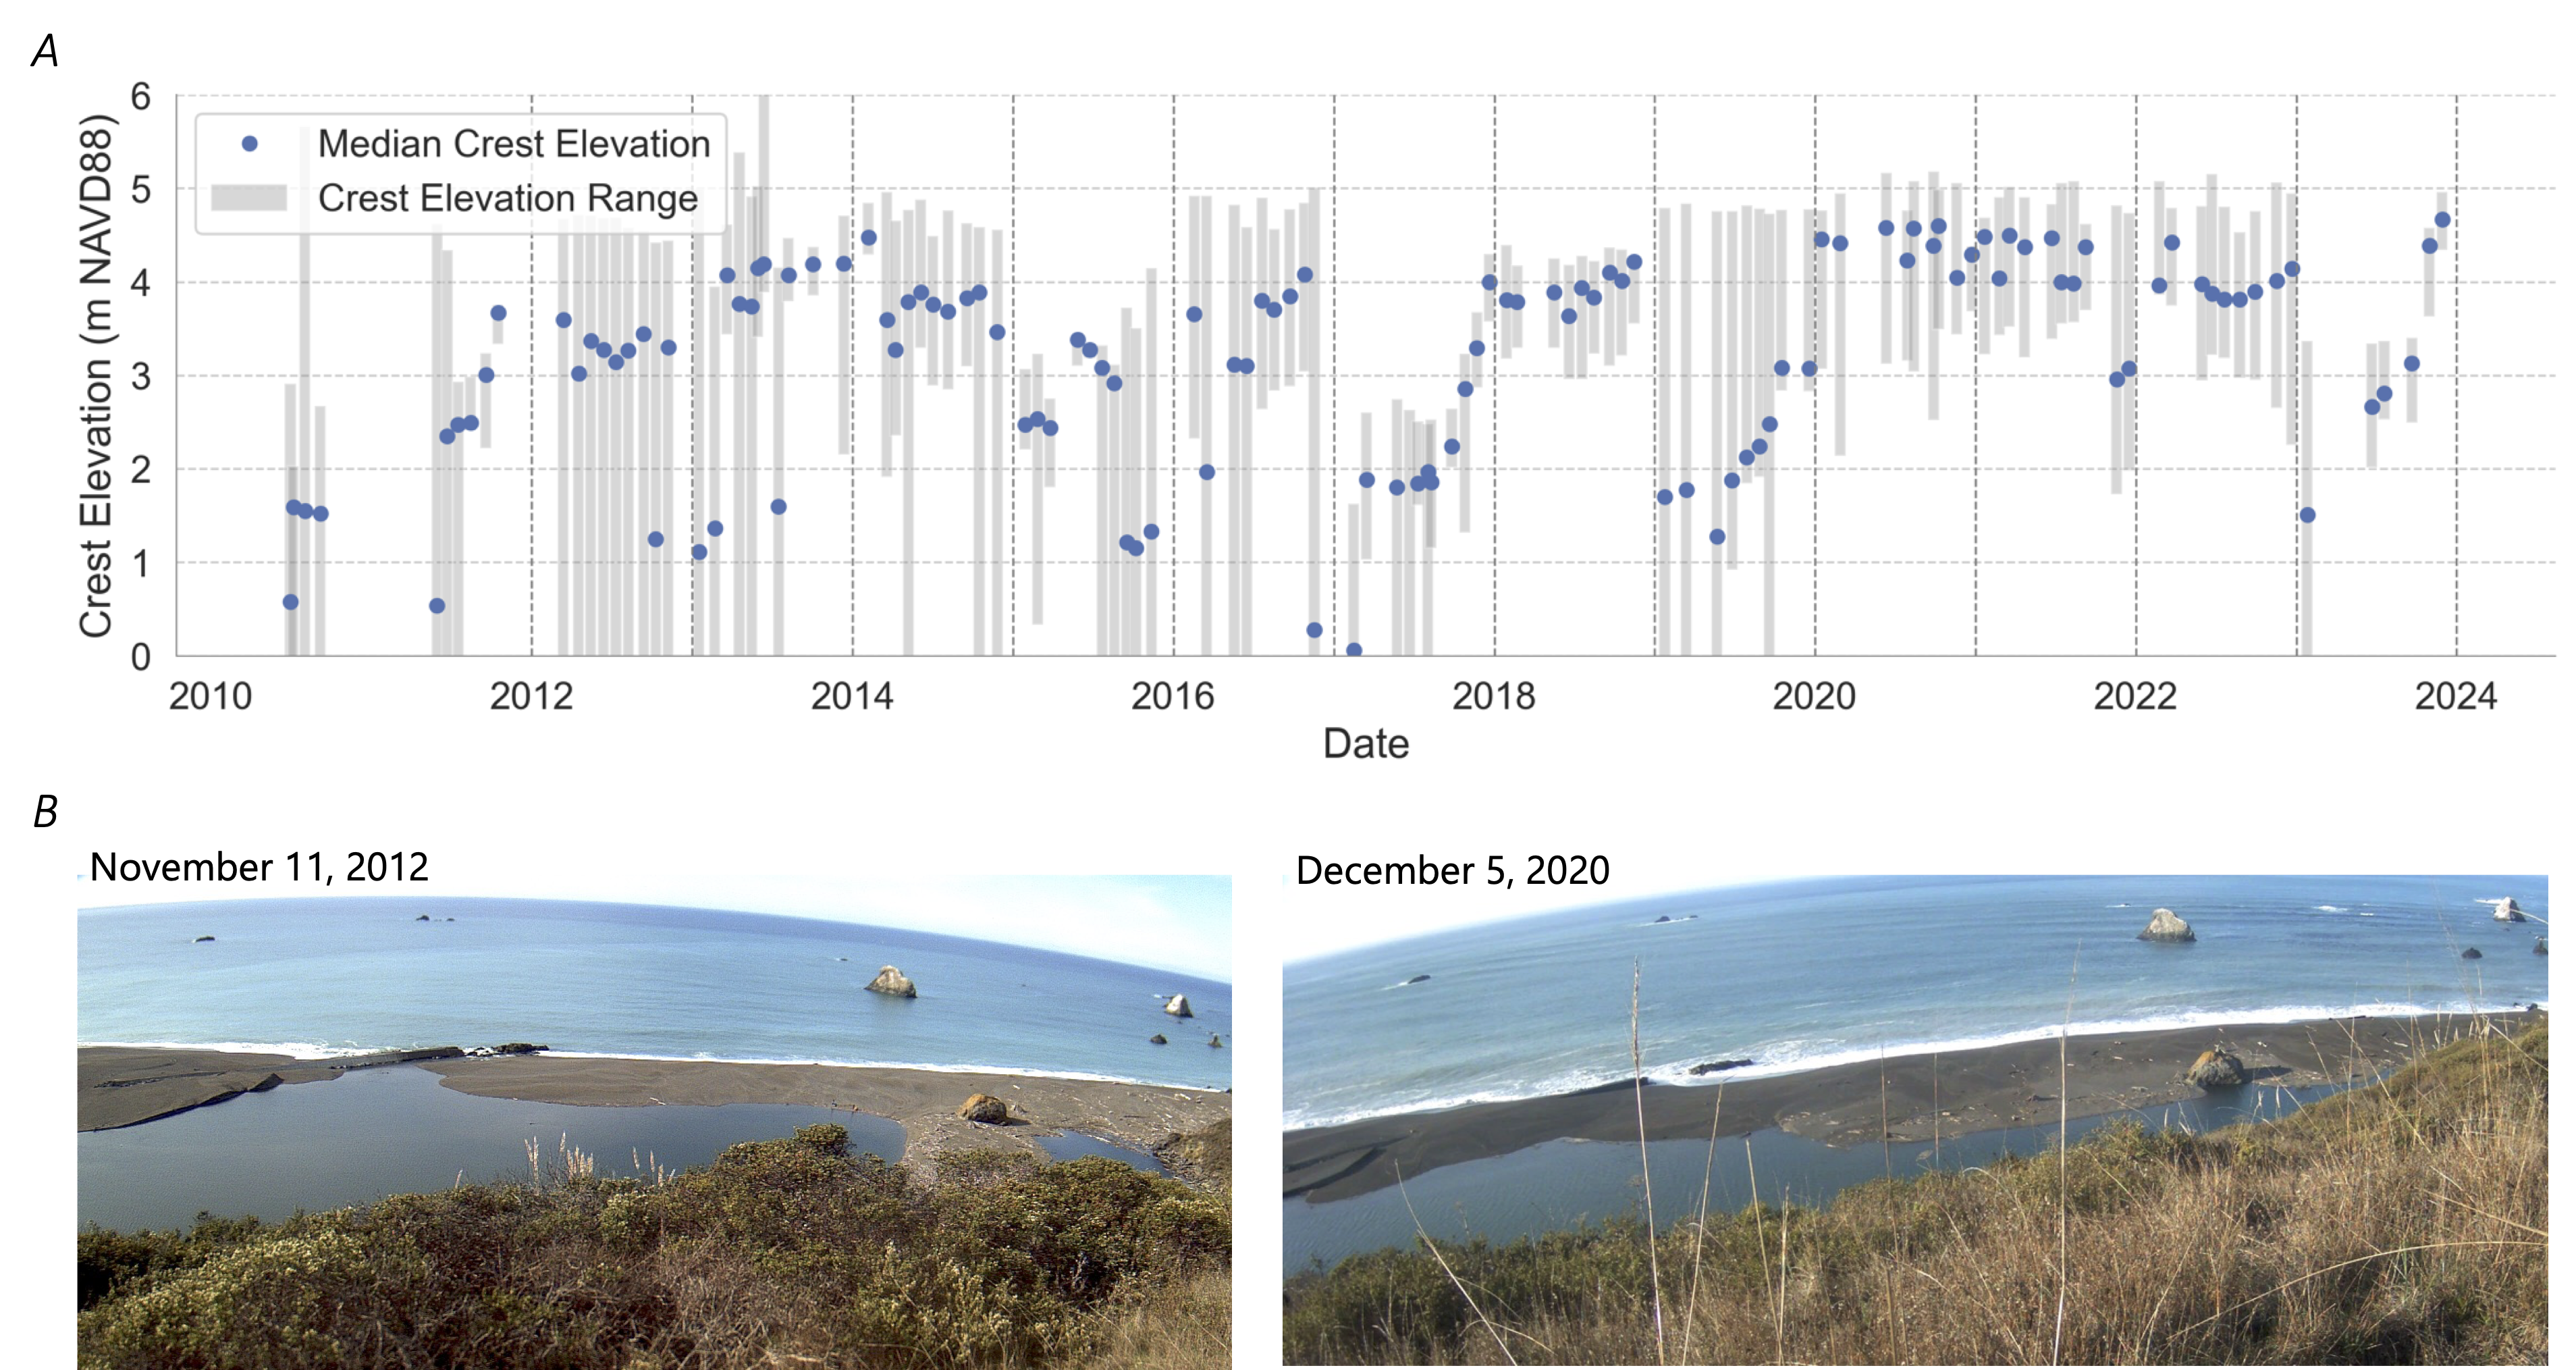
\includegraphics[width = \textwidth]{figures/interannual_variability.png}
    \caption{Berm crest elevation as a function of time, showing the median (blue dots) and range of  four transects across the berm. Photos taken on November 11, 2012 and December 5, 2020, illustrating larger interannual changes in the berm shape.  In 2012, large $C_L$ is consistent with a narrowing berm by the jetty.  Likewise, in 2020, small $C_L$ is consistent with the wider berm shape.   }
    \label{fig:berm_crest}
\end{figure}

  \begin{figure}
    \centering
    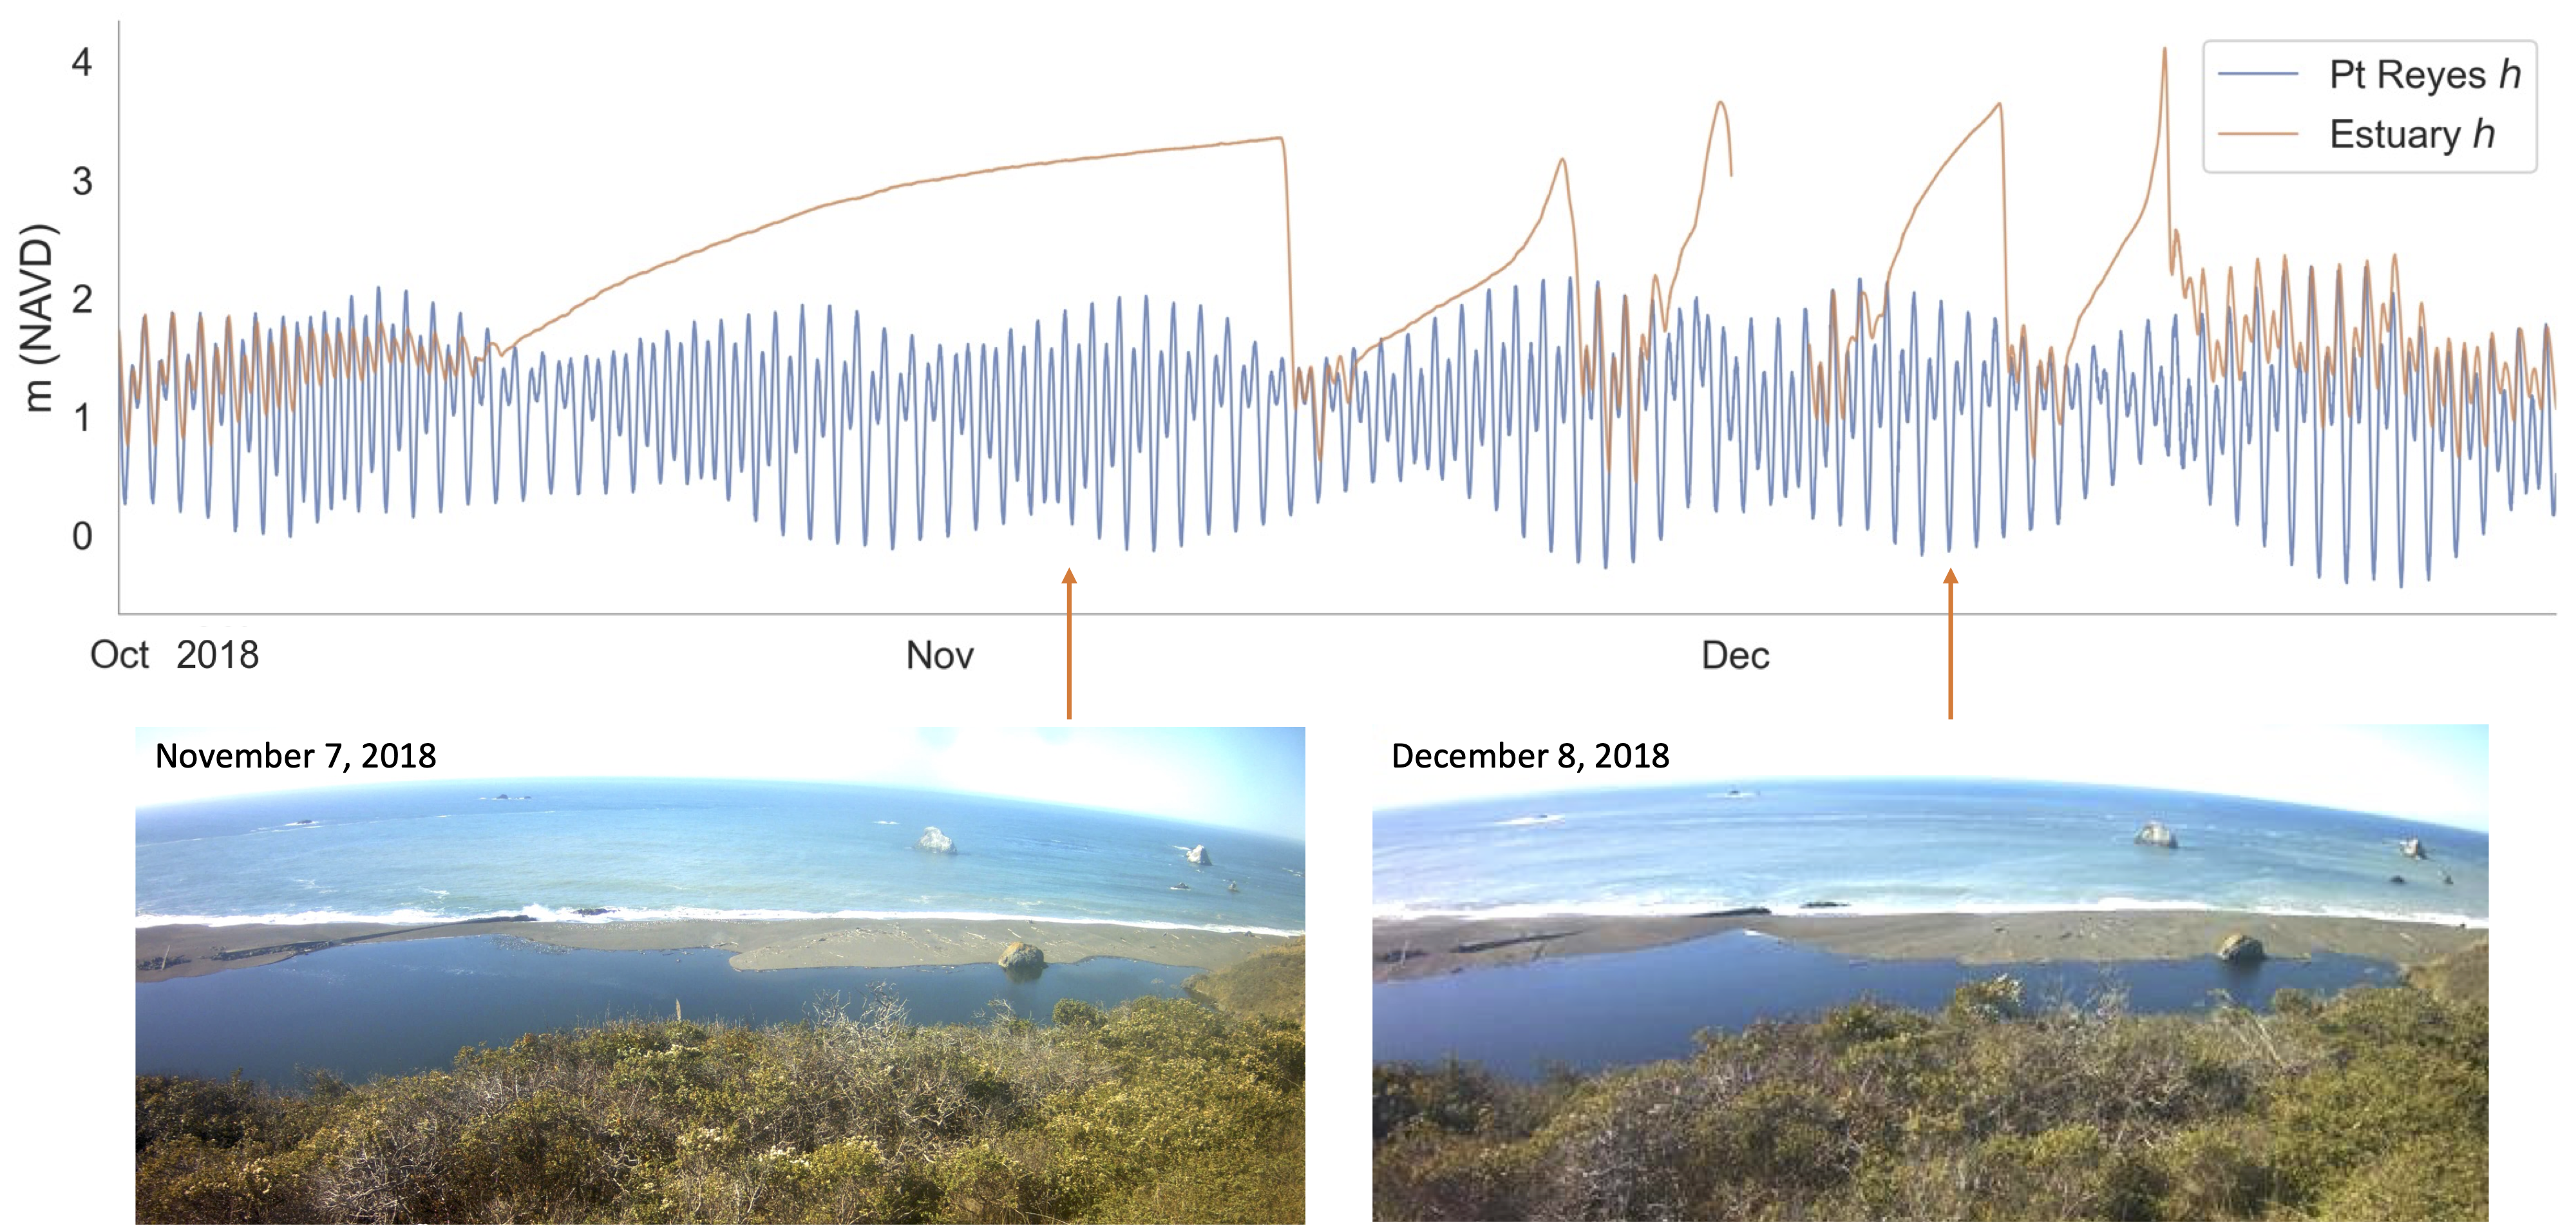
\includegraphics[width = \textwidth]{figures/subsequent_closures.png}
    \caption{Photos taken November 7, 2018 and December 8, 2018, illustrate how the berm shape varies little over subsequent closures within the same year. }
    \label{fig:2018_closures}
\end{figure}

In the absence of wave overwash,  day-to-day variability in $S$ is on the order of 0.1 m$^3$/s, which is an order of magnitude smaller than typical seepage rates. More persistent sources of uncertainty in seepage estimates include:
(i)  evaporative loss from the estuary,
(ii) unaccounted for wave overwash events,
(iii) groundwater exchange, and
(iv) differences in ocean water level between Point Reyes gauge and the Russian River mouth associated with wind and wave setup.
We assessed whether errors in ocean level estimates due to wind or wave setup could  explain outliers in $S$ estimates, and found no clear relationship with short-lived wind or wave events that may account for local water level setup.
While unlikely to change the above-described mass balance that exhibits a tight relation between head and through-berm seepage, the role of groundwater fluxes remains an uncertainty in general and it may be an important term in other intermittently closed estuaries.

With the observed seepage rates and dependence on estuary water level, a steady-state balance could occur in the Russian River estuary (i.e., where river inflow is balanced by seepage through the berm, allowing for persistent closures). The berm is often high enough for estuary water level to rise 2-3 m above ocean water levels. Under these conditions, seepage could be as high as 2 or 3 m$^3$/s (100-140 cfs, using overall best-fit value for $C_L$ of 1.07; Figure 5D), which is greater than typical summer river flow rates that are managed to maintain adequate water availability in the lower river.
However, this steady state is rarely achieved, because
the estuary mouth is breached mechanically before estuary water level reaches 2.74 m NGVD29 (1.9 m NAVD), limiting the maximum seepage rates.
At this level, seepage can account for a loss of approximately 2 m$^3$/s, which is less than typical summer river flows. An exception is in the 2014 drought year, when river flow rate decreased to  approximately 2 m$^3$/s and long closures were observed (Table 1). For the first 10 days of October, seepage balanced river inflow and the water level remained nearly constant in the estuary increasing $\approx$0.2 m from 2.7 to 2.9 m NAVD (see Figure \ref{fig:overwash}).

Steady-state conditions likely occurred prior to human modifications, as closures could start in spring and persist for months through the summer low-flow months. Alternatively, closure may have persisted with the estuary water level over-topping the crest of the berm (i.e., perched state), but with high seepage allowing for an overflow rate low enough that the berm was not scoured. For example, in this perched estuary state, if 0.5 m$^3$/s flowed over the sand barrier as a 10 m wide and 0.1 m deep flow with velocities below 0.5 m/s, flow would likely  not scour the sand and the barrier would remain in place.

Prolonged closures allow a freshwater layer (epilimnion) to develop in the estuary, which offers critical habitat for freshwater-acclimated young steelhead \citep{largier20205}. Further, a cool, moderate-salinity metalimnion also can develop, offering habitat for smolts to grow prior to leaving the estuary and entering the ocean in the fall. The deep and cold hypolimnion becomes anoxic beneath very strong stratification that precludes mixing and re-oxygenation, without any significant photosynthetically active radiation. If the present management protocol continues under rising sea level, the maximum head difference between estuary and ocean will be reduced, and the maximum possible seepage will be further constrained.  This may result in shorter closure events, with less persistent and thinner epilimnion and metalimnion layers, reducing valuable habitat for juvenile salmonids. Because seepage is a first-order term in the closed-estuary water balance, an explicit, head-dependent estimate of it has the potential to improve operational forecasts of how quickly water level rises toward the breaching threshold, and hence the timing of managed breaches that trade flood risk against habitat value. The same head-dependence implies that sea-level rise will reduce the seepage that drains the estuary during closures, so maintaining the long closures that support salmonid habitat may increasingly depend on the management options actually available, namely the volume and timing of managed inflow and the threshold at which the berm is artificially breached.

 Seepage losses are likely significant in other ICEs where the water level rises significantly above the ocean water level, which occurs where river inflow exceeds evaporative losses during closure periods.  Different barrier configurations, in terms of dimensions and sediment types, are expected to result in different flow rates.  Likewise, other ICEs may exhibit differences in how $C$ changes over seasons and years, due to clogging and/or changes in berm shape. While some data exist for similar water-balance analyses in other California ICEs, new work should also include data collection that can better define and demonstrate controls on the seepage process.

\label{sec:discussion}

\section{Conclusion}

This study combined a multi-year record of the daily condition of the Russian River inlet, estuary water level, and river discharge data to compute seepage rates during estuary closures.
We then estimated an integrated hydraulic conductance $C_L$ by regression of the seepage rate $S$ on the head difference between ocean and estuary, $\Delta h$.
Aggregating over 32 closure events with at least five daily data points ($N \ge 5$), we find that the average seepage rate is $S = 1.07\,\Delta h$.
We suggest that interannual variability in $C_L$ reflects variations in berm shapes, and seasonal variability reflects changes in the composition and hydraulic conductance of the berm (e.g., clogging by fine particles).


\section{Acknowledgments}
We are grateful for funds and data received from the Sonoma County Water Agency to UC Davis Bodega Marine Laboratory and Environmental Science Associates for monitoring of estuary conditions in the Russian River. UC Davis is also grateful for funds received from the California Department of Parks and Recreation for monitoring and understanding water levels in Californian estuaries. The authors thank Jessica Martini-Lamb, Chris Delaney, Michael Koohafkan, and Elinor Twohy for dialog, insight, and assistance in this study.



 \bibliographystyle{elsarticle-harv}
 \bibliography{local.bib}

\end{document}